\chapter{Introducción}	

Las redes profundas han demostrado ser modelos de aprendizaje automático muy efectivos, proporcionando resultados correspondientes al estado del arte (véase \cite{Goodfellow-et-al-2016} y \cite{LeCun-Yann-Bengio}) en gran variedad de tareas como segmentación, clasificación de imágenes o el reconocimiento automático de voz. Una de las arquitecturas de este tipo con mayor éxito son las redes convolucionales, que prevalecen en los problemas de visión por computador. Las redes convolucionales modernas están formadas por capas consecutivas, donde cada capa aplica un operador lineal convolucional, definido por unos pesos, seguido de una Unidad Lineal Rectificada (ReLu) como función de activación que está definida como $\sigma(x) = max\{x,0\}$ para un valor de entrada $x \in 
\mathbb{R}$ seguida por \textit{max} o \textit{average pooling}. \textit{Max pooling} está definido como $P\{c_j\}=max\{c_j\}$ para un conjunto de valores $\{c_j\}$ y \textit{average pooling} como $P\{c_j\}=mean\{c_j\}$. Dichos modelos serán llamados \textbf{redes convolucionales rectificadoras}. 

El conocimiento teórico sobre este tipo de redes es menor. Se cree que gozan de \textbf{eficiencia en profundidad}, es decir, cuando son profundas (tienen muchas capas) pueden implementar con tamaño polinomial (en el número de convoluciones) computaciones que necesariamente necesitan de tamaño super-polinomial (en el número de convoluciones) para implementarse en una red es poco profunda. En el caso en que esto ocurra para una red para todos los pesos posibles de sus convoluciones, salvo un conjunto de medida nula, se dirá que goza de \textbf{eficiencia en profundidad completa}. Se cree que las redes convolucionales rectificadoras gozan de eficiencia en profundidad, pero hay pocos argumentos formales que indiquen esto. Además no está claro hasta que punto las redes convolucionales rectificadoras aprovechan la eficiencia en profunidad, esto es, para qué proporción de los pesos posibles se cumple que la red poco profunda requiere tamaño super-polinomial para implementar el mismo cálculo.


Por otro lado se tiene un mejor entendimiento teórico sobre la eficiencia en profundidad para los circuitos aritméticos, en particular para los circuitos aritméticos convolucionales. Los \textbf{circuitos aritméticos} son redes con dos tipos de nodos: nodos suma, que calculan una suma ponderada de las entradas a dicho nodo, y los nodos producto, que calculan el producto de sus entradas. La eficiencia en profundidad de estas redes ha sido estudiada en profundidad al contrario que para las redes convolucionales. Los \textbf{circuitos aritméticos convolucionales} son una subclase de los circuitos aritméticos. Específicamente estos son redes convolucionales con función de activación lineal ($\sigma(x) = x$) y \textit{product pooling} ($P\{c_j\} = \prod c_j$). Se sabe que este tipo de redes gozan de eficiencia en profundidad completa.

En este TFG se utiliza una construcción, basada en la noción de \textbf{factorización generalizada de tensores}, utilizada en \cite{DBLP:journals/corr/CohenSS15a} que transforma circuitos aritméticos convolucionales en redes convolucionales rectificadoras. Después se utilizarán las herramientas matemáticas previamente utilizadas para probar resultados sobre circuitos aritméticos para probar resultados sobre la expresividad y eficiencia en profundidad de redes rectificadoras. 

En concreto se verá que las redes convolucionales rectificadoras con \textit{pooling average} no son universales (hay funciones que no pueden implementar) mientras que las redes convolucionales rectificadoras con \textit{max pooling} y los circuitos aritméticos convolucionales sí lo son. Para los dos últimos casos se tendrá que ambas redes cumplen la eficiencia en profundidad, aunque únicamente los circuitos aritméticos convolucionales gozan de eficiencia en profundidad completa. Dichos resultados indican que dentro de las dos redes convolucionales rectificadoras, se tiene mayor expresividad y eficiencia en profundidad con \textit{max pooling} comparado con el operador de \textit{pooling average}. Por otro lado, la diferencia en la completitud de la eficiencia en profundidad entre la red convolucional rectificadora con \textit{pooling} del máximo y el circuito aritmético convolucional, indica que los circuitos aritméticos convolucionales obtienen mayor beneficio de tener más capas. 

Finalmente se verá la eficiencia en profundidad desde el punto de vista de aproximar los cómputos de la red profunda mediante la red poco profunda, en vez de la realización exacta.

Todos los capítulos de esta parte siguen el esquema utilizado en la publicación \cite{DBLP:journals/corr/CohenS16} y muchos de los resultados son de dicho trabajo. Los resultados que provengan de otras fuentes serán citados acordemente.

Por lo tanto este TFG va a seguir el siguiente esquema. En primer lugar se introducirá el concepto de tensor y de factorización generalizada de tensores. Luego se introducirán la arquitectura de la redes que se van a estudiar y un tensor asociado a dichas redes, el \textbf{tensor cuadrilla}, que permitirá el estudio de estas redes. Después se realizará el estudio teórico de las redes, tanto sobre la expresividad de estas como de eficiencia en profundidad, para dos casos cuando los pesos son compartidos y cuando no lo son. Para ello se introducirá una serie de resultados auxiliares previos que se utilizarán a lo largo del estudio y se explicará qué es la matrificación de un tensor, lo que permitirá usar resultados sobre matrices para el estudio de las propiedades de las redes. 
\newpage 

\chapter{Factorización generalizada de tensores}
En este capítulo se define qué es un tensor y cuáles son sus operadores más importantes. También se introduce la notación que se utilizará y finalmente se verá qué es una factorización de un tensor. Las definiciones, operadores y notación introducidas en este capítulo se han sacado principalmente de \cite{DBLP:journals/corr/CohenS16}, \cite{libro} y \cite{doi:10.1137/07070111X}.

Para los propósitos de este trabajo se definirá un tensor como la generalización de los conceptos de vector y matriz, que se puede encontrar en la sección 1.1.1 de \cite{libro}. Cabe destacar que hay una definición más formal de tensor que se puede consultar en la sección 3 de \cite{libro}.

\begin{definicion}
Un \textbf{tensor} es un array multidimiensional que toma valores en $\mathbb{R}$ en cada entrada. La entrada de un \textbf{tensor} A en los índices $d_1,d_2,...,d_N$ se denotará como $A_{d_1,d_2,...,d_N}$. Un \textbf{tensor} se puede definir a través de los valores que toma en cada entrada.
\end{definicion}

\begin{definicion}
Sea A un tensor. Se define el \textbf{orden} de A como el número de índices del tensor. 
\end{definicion}

\begin{definicion}
Cada uno de los índices de un tensor se denominará \textbf{modo}. 
\end{definicion}

\begin{definicion}
La \textbf{dimensión} de un modo de un tensor es el número de valores posibles que puede tomar dicho modo.
\end{definicion}

Sea un tensor $A\in\mathbb{R}^{M_1\times M_2 \times \cdots \times M_N}$ que toma los valores:

$$ A_{d_1,..,d_N}\in\mathbb{R}\quad,d_i\in[M_i]=\{1,...,M_i\}, \;\; i=1,...,N
$$

Entonces $A$ tiene orden $N$, por lo tanto tiene $N$ modos. La dimensión correspondiente al modo $i\in\{1,2,...,N\}$ es $M_i\in\mathbb{N}$. En particular, cuando $N=1$ se obtiene un vector mientras que si $N=2$ se obtiene una matriz.

\begin{ejemplo} \label{ej:tensorejemplo}
Consideramos $A$ el tensor de orden $3$ y con dimensiones $M_1 = 2, M_2 = 3$ y $M_3 = 2$ que toma los siguientes valores: 
\begin{align*}
&A_{1,1,1} = 1 \quad A_{1,2,1} = 2 \quad A_{1,3,1} = 3 \quad A_{2,1,1} = 4 \quad A_{2,2,1} = 5 \quad A_{2,3,1} = 6 \\
&A_{1,1,2} = 7 \quad A_{1,2,2} = 8 \quad A_{1,3,2} = 9 \quad A_{2,1,2} = 10 \quad A_{2,2,2} = 11 \quad A_{2,3,2} = 12 \\ 
\end{align*}

Si se fija el índice, $k$, del último modo se pueden ver los valores del tensor anterior para dicho índice fijo como una matriz que en la fila $i$ y columna $j$ toma el valor $A_{i,j,k}$. Dicha matriz se denotará $A_{:,:,k}$ para el índice fijo $k$. Por lo tanto el tensor $A$ del ejemplo queda definido por las siguientes matrices:

\begin{align*}
A_{:,:,1} = \begin{bmatrix}
1 & 2 & 3 \\
4 & 5 & 6 
\end{bmatrix} \quad
A_{:,:,2} = \begin{bmatrix}
7 & 8 & 9 \\
10 & 11 & 12 
\end{bmatrix}
\end{align*}

Evidentemente esto se puede realizar fijando cualquiera de los tres índices. Por ejemplo se podría expresar el tensor mediante 3 matrices $2\times 2$ cada una correspondiente a fijar el segundo índice a un valor distinto.
\end{ejemplo}

Las operaciones de tensores introducidas a continuación serán las que se utilizarán principalmente a lo largo del trabajo.

\begin{definicion}
Sean $A\in\mathbb{R}^{M_1\times \cdots \times M_P}$ y $B\in\mathbb{R}^{M_1\times \cdots \times M_P}$ dos tensores que comparten el orden y tienen la misma dimensión en sus modos. Entonces se define su \textbf{suma}, denotada por $A+B\in\mathbb{R}^{M_1\times\cdots \times M_P}$, cómo el tensor que tiene mismo orden y misma dimensión en cada uno de sus modos que $A$ y $B$, cuyos valores son los siguientes:
\begin{equation}
(A + B)_{d_1,..,d_{P}} = A_{d_1,..,d_P} + B_{d_1,..,d_P} \quad, d_i\in[M_i], \;\; i=1,\cdots ,P
\end{equation}

Es decir, la suma elemento a elemento.

\end{definicion}

\begin{definicion}
Se define el \textbf{producto tensorial}, denotado por $\ttimes$, como el operador que para dos tensores cualesquiera $A\in\mathbb{R}^{M_1\times\cdots \times M_P}$ y $B\in\mathbb{R}^{M_{P+1}\times\cdots \times M_{P+Q}}$ con $P,Q\in\mathbb{N}$ devuelve como salida el tensor $(A\ttimes B) \in\mathbb{R}^{M_1\times\cdots \times M_{P+Q}}$ cuyos valores son los siguientes:

\begin{equation}
(A\ttimes B)_{d_1,..,d_{P+Q}} = A_{d_1,..,d_Q} \cdot B_{d_{P+1},..,d_{P+Q}}\quad, d_i\in[M_i], \;\; i=1,\cdots ,P+Q
\end{equation}
\end{definicion}

\begin{ejemplo}
Sean los siguientes tensores $A$ y $B$ definidos como sigue:

\begin{align*}
A = \begin{bmatrix}
1 & 2 & 3 \\
4 & 5 & 6
\end{bmatrix} \quad y \quad 
B = \begin{bmatrix}
1 \\
2 \\
\end{bmatrix}.
\end{align*}

En particular se tiene que $A$ es una matriz y $B$ un vector. Entonces su producto tensorial $C = A \ttimes B$ queda definido por las siguientes dos matrices:

\begin{align*}
C_{:,:,1} = \begin{bmatrix}
1 & 2 & 3 \\
4 & 5 & 6 
\end{bmatrix} \quad
C_{:,:,2} = \begin{bmatrix}
2 & 4 & 6 \\
8 & 10 & 12 
\end{bmatrix}
\end{align*}

\end{ejemplo}

El producto tensorial cumple la siguiente propiedad:

\begin{prop} \label{prop:prodtensasociativo}
El producto tensorial es asociativo.
\end{prop}
\begin{proof}
Sean los tensores $A\in\mathbb{R}^{M_1\times\cdots \times M_P}$, $B\in\mathbb{R}^{M_{P+1}\times\cdots \times M_{P+Q}}$ y $C\in\mathbb{R}^{M_{P+Q+1}\times\cdots \times M_{P+Q+L}}$ entonces para $d_i\in[M_P]$ para todo $i\in[P+Q+L]$ se cumple que:

\begin{align*}
((A\ttimes B)\ttimes C)_{d1,d2,\cdots ,d_{P+Q+L}} &= (A_{d_1,..,d_Q} \cdot B_{d_{P+1},..,d_{P+Q}}) \cdot C_{d_{P+Q+1},\cdots ,d_{P+Q+L}} \\ 
	&= A_{d_1,..,d_Q} \cdot (B_{d_{P+1},..,d_{P+Q}} \cdot C_{d_{P+Q+1},\cdots ,d_{P+Q+L}}) \\
	&= (A\ttimes (B\ttimes C))_{d1,d2,\cdots ,d_{P+Q+L}}
\end{align*}
\end{proof}

Se denotará por $\ttimes_{i=1}^{N} A_i$ para $N\in \mathbb{N}$ tensores, al producto tensorial de dichos tensores, esto es:

$$
\ttimes_{i=1}^{N} A_i = A_1 \ttimes A_2 \ttimes \cdots  \ttimes A_N
$$

De igual forma se denotará como $\sum_{i=1}^{N} A_i$ a la suma de $N$ tensores, que será posible únicamente si tienen iguales órdenes y dimensiones dichos tensores.

Para los propósitos del trabajo se utiliza la siguiente generalización del producto tensorial:

\begin{definicion} \label{def:factorizacionGeneralizada}
Sea $g:\mathbb{R}\times\mathbb{R}\rightarrow\mathbb{R}$ un operador binario conmutativo y asociativo. Se define el \textbf{producto tensorial generalizado}, denotado por $\gtimes$, como el operador que para dos tensores cualesquiera $A\in\mathbb{R}^{M_1\times\cdots \times M_P}$ y $B\in\mathbb{R}^{M_{P+1}\times\cdots \times M_{P+Q}}$ con $P,Q\in\mathbb{N}$ devuelve como salida el tensor $(A\gtimes B) \in\mathbb{R}^{M_1\times\cdots \times M_{P+Q}}$ cuyos valores son los siguientes:

\begin{equation}
(A\ttimes_g B)_{d_1,..,d_{P+Q}} = g(A_{d_1,..,d_Q},B_{d_{P+1},..,d_{P+Q}})\quad, d_i\in[M_i], \;\; i=1,\cdots ,P+Q
\end{equation}

\end{definicion}

Obsérvese que el producto tensorial generalizado con el operador binario $g(a,b) = a \cdot b$ es el producto tensorial usual. La proposición \ref{prop:prodtensasociativo} también se cumple para el producto tensorial generalizado con cualquier operador $g$ (la demostración es idéntica a la dada).

Una \textbf{factorización de un tensor} es un esquema que sirve para expresar tensores mediante una combinación de productos tensoriales y sumas ponderadas de otros tensores. Una \textbf{factorización generalizada de un tensor} es una factorización de un tensor en la que se utiliza el producto tensorial generalizado $\ttimes_g$ en lugar del producto tensorial $\ttimes$. El producto tensorial generalizado se utilizará para expresar tensores que permiten el estudio de redes convolucionales mediante factorizaciones generalizadas. En el siguiente capítulo se verán las dos factorizaciones que se usarán en este trabajo.


\newpage
\chapter{Transformación de redes a tensores}

En este capítulo se describirá cómo es la arquitectura de las redes analizadas y se verá qué parámetros tienen. Luego se introducirá el concepto de tensor cuadrilla para una red y se dará una factorización generalizada de este para una red profunda y para una poco profunda. La estructura de la red convolucional que se va a estudiar se puede ver en la figura \ref{fig:red_convolucional_estrucutra}. 


\begin{figure}[h]
\noindent
\makebox[\textwidth]{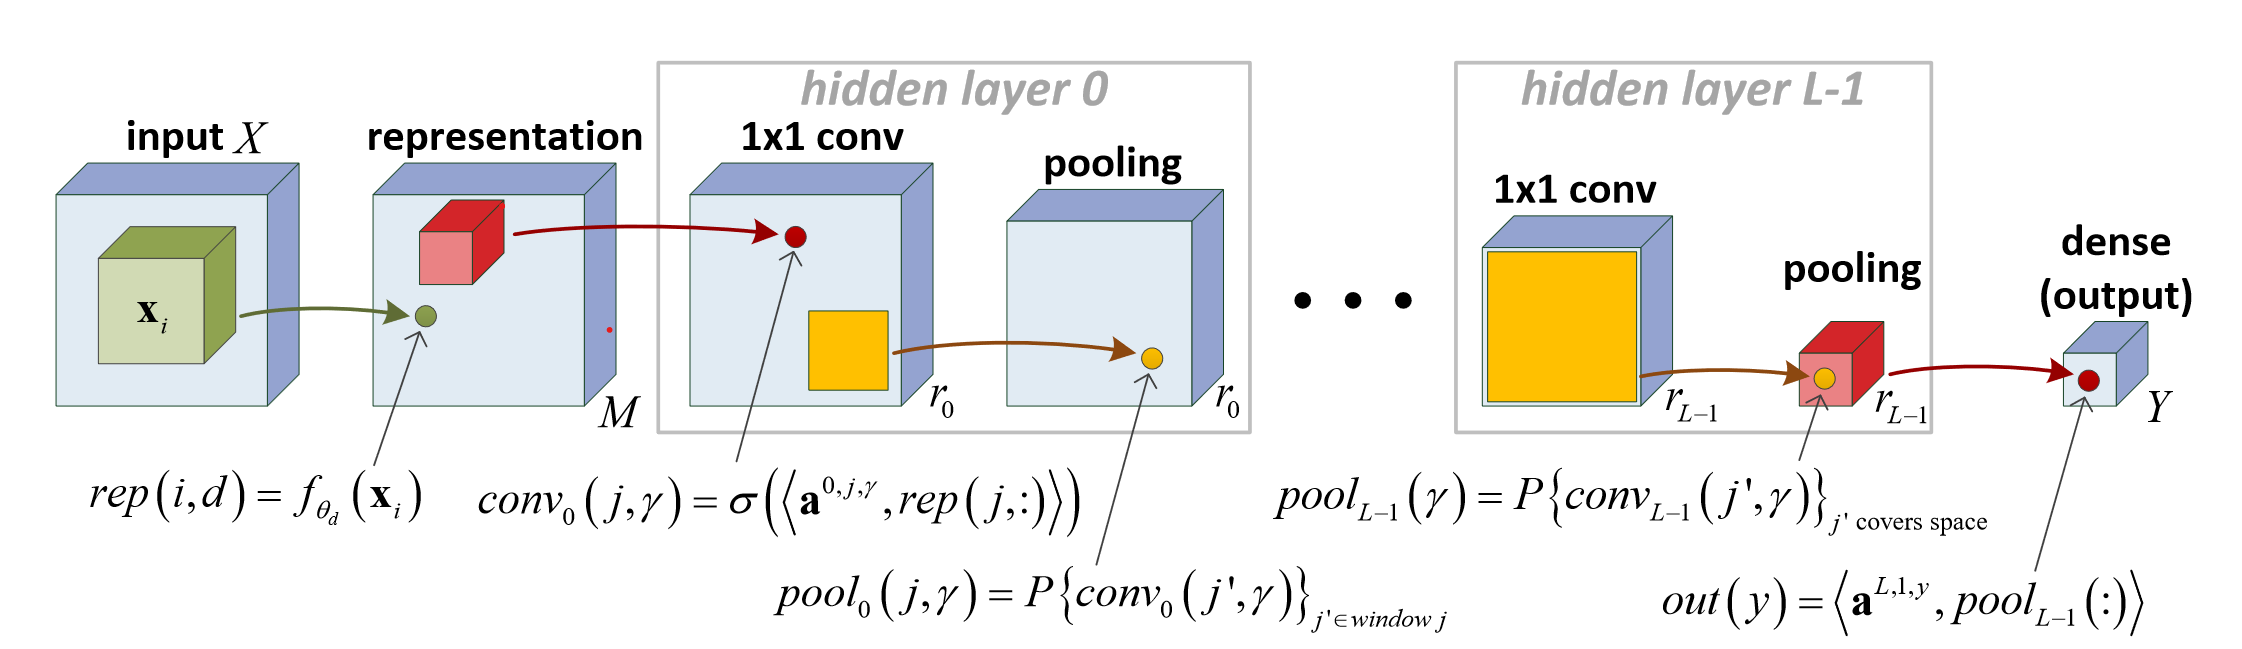
\includegraphics[scale=0.36]{images/RedConvEstudiada}}
\caption{Estructura de la arquitectura de la red utilizada. Se puede ver el flujo de los datos desde la entrada hasta la salida. Primero se aplican las funciones de representación, después las $L-1$ capas ocultas aplican cada una la convolución, seguida de la función de activación y el \textit{pooling}, y finalmente se aplica la capa totalmente conectada. Imagen extraída de \cite{DBLP:journals/corr/CohenS16}}.
\label{fig:red_convolucional_estrucutra}
\end{figure}

La entrada a la red, representada por $X$, consistirá en $N\in\mathbb{N}$ \textbf{parches} $\bx_1,\cdots ,\bx_N\in\mathbb{R}^s,\; s\in \mathbb{N}$. Por ejemplo, si se tiene una imagen RGB de $10\times10$ píxeles donde cada píxel tiene asociado tres valores (rojo, verde, azul) y cada parche abarca una región $5\times5$ que se escoge alrededor de cada píxel (los píxeles fuera de la imagen se toman como $(0,0,0)$). Entonces en el modelo se tendría $X$ con $N=100$ parches y con $s=5\cdot5\cdot3=75$. La primera capa de la red, referida como \textbf{capa de representación}, consiste en aplicar $M\in\mathbb{N}$ \textbf{funciones de representación} $f_{\theta_1},\cdots ,f_{\theta_M}:\mathbb{R}^s\rightarrow\mathbb{R}$ a cada uno de los parches de entrada, formando $M$ \textbf{mapas de características}. Estas funciones dependen de un parámetro $\theta_i$ que toma valores en un conjunto $\Theta$, que dependerá de las funciones de representación elegidas. Siguiendo el ejemplo anterior, cada mapa de características se puede ver como una matriz con valores en $\mathbb{R}$ y con las mismas dimensiones que la imagen de entrada, que en cada posición tiene el resultado de aplicar al parche de $X$ correspondiente al píxel en dicha posición de la imagen de entrada la función de representación correspondiente a este mapa de características. Por lo tanto la salida de esta primera capa, en el ejemplo, se puede ver como un tensor de tres modos, denótese por $R$, donde el tercer modo tiene dimensión $M$ (este es el número de \textbf{canales} de la salida de la capa de representación) y que para cada $m \in \{1,2\cdots ,M\}$ (cada canal) se tiene que $R_{:,:,m}$ es el mapa de características correspondiente a $f_{\theta_m}$.

Antes de explicar las siguientes capas conviene remarcar que cuando se habla de aplicar una convolución, se está hablando de aplicar una convolución discreta en dos dimensiones (definición sacada de \cite{Goodfellow-et-al-2016}).

\begin{definicion} \label{def:operadorConvolucion}
Sean $f,g:\mathbb{Z}\times\mathbb{Z}\rightarrow\mathbb{R}$, se define la \textbf{convolución discreta} de f y g como:
\begin{equation}
(f\star g)[i,j] = \sum_{m=-\infty}^{\infty}\sum_{n=-\infty}^{\infty}f(m,n)g(i-m,j-n)
\end{equation}

A $g$ se le llamará \textbf{núcleo} o \textbf{filtro}.
\end{definicion} 

En particular, las redes convolucionales aplican convoluciones discretas con soporte finito, es decir, $g$  tendrá valores distintos de $0$ en un rango de valores de $\{-m,\cdots ,m\}\times\{-n,\cdots ,n\}$ con $m,n\in\mathbb{N}$, en cuyo caso se dirá que se tiene una convolución $(2 \cdot m + 1) \times (2 \cdot n + 1)$. A los valores que toma $g$ se le llaman \textbf{pesos} de la convolución (o pesos del filtro). 

En el caso de la arquitectura estudiada, las salidas de las capas se pueden ver como tensores de orden 3, donde la dimensión del tercer modo se dice que es el número de canales. Por lo tanto, cuando se hable de aplicar una convolución a la salida de una capa, lo que se hace es aplicar una convolución discreta distinta a cada canal y se suma el resultado de cada uno de estos. Por ejemplo si se aplica una convolución $g$ $1\times 1$ a un tensor $A$ que tiene $K$ canales, se tiene que:
\begin{align} \label{eq:filtroAplicado}
(f\star g)[i,j] = \sum_{k=1}^{K}f_k(i,j)g_k(0,0)
\end{align}

Donde $f_k(i,j) = A_{i,j,k}$ y $g_k$ representa los pesos de la convolución que se aplica al canal $k$.

Así que de ahora en adelante, cuando se hable de aplicar una convolución $1\times 1$, basta con dar un vector de pesos de dimensión igual al número de canales del tensor al que se aplica.

\begin{ejemplo}
Sea $A\in\mathbb{R}^{2\times 3 \times 2}$ el tensor definido por:
\begin{align*}
A_{:,:,1} = \begin{bmatrix}
1 & 2 & 3 \\
4 & 5 & 6 
\end{bmatrix} \quad
A_{:,:,2} = \begin{bmatrix}
7 & 8 & 9 \\
10 & 11 & 12 
\end{bmatrix}
\end{align*}

Y sea el filtro con pesos $\ba\in\mathbb{R}^2$:

\begin{align*}
\ba = \begin{bmatrix}
2 \\
1 \\
\end{bmatrix}
\end{align*}

El resultado de aplicar dicha convolución a $A$ es la siguiente matriz:

\begin{align*}
\begin{bmatrix}
1\cdot 2 + 7\cdot 1 & 2\cdot 2 + 8\cdot 1 & 3\cdot 2 + 9\cdot 1 \\
4\cdot 2 + 10\cdot 1 & 5\cdot 2 + 11\cdot 1 & 6\cdot 2 + 12\cdot 1
\end{bmatrix}
=
\begin{bmatrix}
9 & 12 & 15\\
18 & 21 & 24
\end{bmatrix}
\end{align*}
\end{ejemplo}


Siguiendo con la estructura de la red, a las funciones de representación le siguen $L\in\mathbb{N}$ \textbf{capas ocultas} indexadas por $l\in\{0,\cdots ,L-1\}$. Cada capa oculta aplica $r_l\in\mathbb{N}$ convoluciones $1\times1$ a la salida de la capa anterior y luego aplica una \textbf{función de activación} $\sigma(\cdot)$, generando un nuevo tensor con las mismas dimensiones en los dos primeros modos y con dimensión $r_l$ en el tercer modo (esta dimensión es el número de canales). Se distinguen dos casos según cómo sean los pesos de cada convolución: el primero donde los pesos de cada filtro serán distintos para cada píxel y el segundo, el estándar, donde el filtro aplica los mismos pesos a todos los píxeles de la entrada. Se denominarán \textbf{caso no compartido} y \textbf{caso compartido}, respectivamente. En el caso en el que los pesos se comparten se corresponde con la definición \ref{def:operadorConvolucion}, mientras que el caso de pesos no compartidos sería igual que en la definición, pero los pesos de $g$ serían dependientes de los valores que tomen $i$ y $j$.


Además de las convoluciones, en cada capa oculta se aplica \textbf{pooling} espacial a cada una de los $r_l$ mapas de características. El \textit{pooling} consiste en aplicar un operador $P(\cdot)$ sobre regiones disjuntas en cada mapa de características, a las que se les denominarán \textbf{ventanas}. Dichas ventanas son una partición del mapa de características y la salida del operador $P$ debe ser un único número. El \textit{pooling} tiene como objetivo reducir las dimensiones espaciales, es decir, las dimensiones de los dos primeros modos del tensor. La última capa oculta realizará \textit{pooling} global, es decir, las ventanas a las que se le aplica el \textit{pooling} son el total del mapa de características, por lo tanto la salida de esta capa es un vector de $r_{L-1}$ valores. Los operadores de \textit{pooling} que se utilizarán en el análisis son el producto cuya salida es el producto de todos los valores de la ventana, la media cuya salida es la media aritmética de todos los valores de la ventana, y el máximo cuya salida es coger el máximo valor de entre todos los valores de la ventana.

Finalmente se aplica una \textbf{capa totalmente conectada} con $Y$ valores de salida. Esto es, cada valor $y$ del vector de salida será una suma ponderada por unos pesos de los valores del vector resultante de aplicar \textit{pooling} global.

Por lo tanto, los valores aprendibles de la red son los siguientes: 

\begin{itemize}
\item[\quad \textbf{-}]\textbf{Pesos de representación:} Estos son los parámetros posibles que pueden tomar las funciones de representación. Se denotan por $\theta_i$ y toman valores en $\Theta$.
\item[\quad \textbf{-}]\textbf{Pesos de las convoluciones:} Cuando se esté en el caso no compartido serán $\ba^{0,j,\gamma}\in\mathbb{R}^{M}$ para la primera capa convolucional y $\ba^{l,j,\gamma}\in\mathbb{R}^{r_{l-1}}$ donde $l\in \{1,2,... ,L\}$ es la capa en la que se realiza la convolución, $j$ la localización a la que se aplica y $\gamma\in\{1,2,... ,r_l\}$ el filtro de esa capa $l$, para el resto de capas. Si se trata del caso compartido es igual pero se omite la localización $j$.
\item[\quad \textbf{-}]\textbf{Pesos de la capa totalmente conectada:} Serán $\ba^{L,1,y}\in\mathbb{R}^{r_{L-1}}$ con $y\in\{1,... ,Y\}$.
\end{itemize}

Así que ya se tienen las herramientas para modelar un circuito aritmético convolucional y una red convolucional rectificadora con \textit{max pooling} o \textit{average}. Para el primer caso se elige la función de activación como $\sigma(x)=x$ (la \textbf{identidad}) y el operador de \textit{pooling} como $P\{c_j\}=\prod c_j$ (el producto de todas las entradas). Para el caso de las redes convolucionales rectificadoras se escoge $\sigma(x)=max\{x,0\}$ (operador \textbf{ReLU}) y el operador del \textit{pooling} será $P\{c_j\}=max\{c_j\}$ (el máximo de todos los valores de la entrada) y $P\{c_j\}=mean\{c_j\}$ (la media aritmética de los valores de entrada), en el caso de \textit{max pooling} y \textit{average pooling} respectivamente.

Para comparar redes profundas con poco profundas se usarán las dos redes más extremas de cada caso. La red poco profunda tendrá \textit{global pooling} en su primera capa oculta, por lo tanto tendrá $L=1$. Esta red se puede ver representada en la figura \ref{fig:red_convolucional_poco_prof}. La red profunda tendrá el mayor número de capas posible. Para ello se elegirá en cada capa oculta, la ventana de \textit{pooling} con tamaño 2 conteniendo valores consecutivos (se recuerda que las ventanas son disjuntas). Por lo tanto se tienen $L=log_2 N$ capas ocultas.

\begin{figure}[h]
\noindent
\makebox[\textwidth]{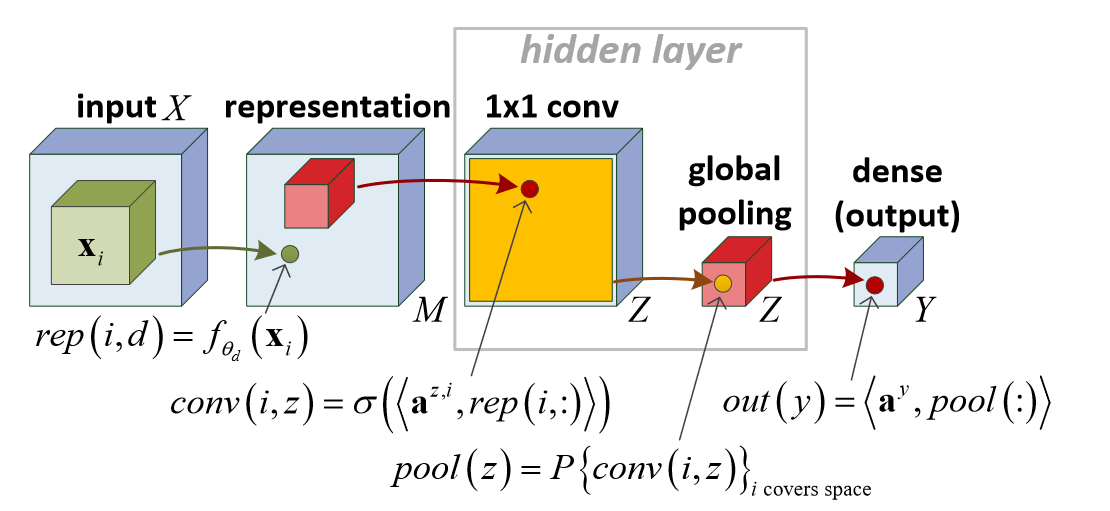
\includegraphics[scale=0.7]{images/RedConvPocoProf}}
\caption{Arquitectura estudiada en el caso de la red poco profunda. Imagen extraída de \cite{DBLP:journals/corr/CohenS16}.}
\label{fig:red_convolucional_poco_prof}
\end{figure}


De aquí en adelante se supone $N$ potencia de $2$ y se denotará como $[n]$ al conjunto $\{1,2,3,... ,n\}$ para cualquier $n\in\mathbb{N}$.

A cada una de las $Y$ salidas de una red se le asocia una función $h_y(\cdot)$ que dependerá de la entrada de la red y devuelve el valor $y\in[Y]$ de la salida red, que es un número real. Para un $y\in[Y]$ específico, a esta función se le denominará \textbf{función de puntuación} para la categoría $y$.

Cuando la red es usada para clasificación, es decir se desea clasificar la entrada en una de las categorías $\{1,2,... ,Y\}$, la clasificación realizada por la red (denotada por $\hat{y}$) para una entrada $X\in(\mathbb{R}^s)^N$ se determina por la siguiente regla:

\begin{align*}
\hat{y}=argmax_{y\in[Y]}h_y(X)
\end{align*}

Dados $M$ vectores fijos $\bx^{(1)},\cdots ,\bx^{(M)}\in\mathbb{R}^s$, denominados \textbf{plantillas}, se define el \textbf{tensor cuadrilla} para una función de puntuación $h_y(\cdot)$ de una red como el tensor de orden $N$ y dimension $M$ en cada modo definido como: 

\begin{equation}
\mathcal{A}(h_y)_{d_1,\cdots ,d_N} = h_y(\bx^{(d_1)},... ,\bx^{(d_N)})
\end{equation}

Es decir, cada entrada del tensor contiene el valor de la función de puntuación para la categoría $y$ cuando la entrada está formada por una combinación específica de las plantillas, pudiéndose repetir el mismo vector en la entrada varias veces.
	
A continuación se van a describir los tensores cuadrilla de cada una de los dos casos de redes que se van a analizar mediante factorizaciones de tensores generalizadas. Para simplifcar la expresión de dichas factorizaciones se define una matriz de dimensiones $M\times M$, denominada por $F \in \mathbb{R}^{M\times M}$, que dependerá de las $M$ funciones de representación de la red. Sean los vectores plantilla fijados anteriormente los mismos, entonces se define $F$ como sigue:


\begin{equation} \label{ec:mf}	
F:=\begin{bmatrix}
f_{\theta_1}(\bx^{(1)}) & \cdots  & f_{\theta_M}(\bx^{(1)})\\
\vdots & \ddots & \vdots\\
f_{\theta_1}(\bx^{(M)}) & \cdots  & f_{\theta_M}(\bx^{(M)})\\
\end{bmatrix}
\end{equation}

Es decir en cada fila $i$ se tiene el vector resultante de aplicar a la plantilla $\bx^{(i)}$ las $M$ funciones de representación.

Antes de ver cómo se expresan los tensores cuadrilla para las redes que se van a analizar, se define el operador $g:\mathbb{R} \times \mathbb{R} \rightarrow\mathbb{R}$ que se utiliza para simplificar las factorizaciones generalizadas que se presentan a continuación. Este operador expresa la activación seguida de \textit{pooling} que sucede en las capas ocultas de la red:

\begin{equation}
	g(x,y)=P(\sigma(x),\sigma(y))
\end{equation}

Donde $P(\cdot)$ es el operador de \textit{pooling} y $\sigma(\cdot)$ es la función de activación para cada red que se vaya a analizar. Se va a comprobar que $g$ cumple las condiciones de la definición \ref{def:factorizacionGeneralizada}. En el caso de circuitos convolucionales aritméticos ($P(a,b)=a\cdot b$ y $\sigma(x)=x$) se cumple pues $g(a,b)=a\cdot b$ que es asociativo y conmutativo pues es el producto usual. En el caso de red convolucional con activación ReLU ($\sigma(x) = max\{x,0\}$) y \textit{max pooling} se tiene que $g(a,b)=max\{max\{a,0\},max\{b,0\}\}=max\{a,b,0\}$ que también es asociativo y conmutativo ya que es el máximo de tres valores. Sin embargo, en el caso de \textit{average pooling} y activación ReLU no se cumple la asociatividad (por ejemplo, no es lo mismo $mean\{mean\{0,1\},1\} = 0.75$ que $mean\{0,mean\{1,1\}\} = 0.5$). Por ello, para analizar estas redes se toma como operador $P$ la suma, es decir, $g(a,b) = max\{a,0\} + max\{b,0\}$. En términos de expresividad esto es equivalente a una red con \textit{average pooling} y activación ReLU ya que el factor multiplicativo que se le ha quitado al operador $g$ se le puede multiplicar a cada valor en los pesos de la siguiente capa.

Ahora, sea el operador $g$ cualquiera de los tres definidos anteriormente y sean $M$ vectores plantilla y funciones de representación, se tiene que el tensor cuadrilla correspondiente al caso de la red poco profunda (con pesos no compartidos) se puede expresar mediante la siguiente factorización:

\begin{equation} \label{fac:tenshal}
\mathcal{A}(h_y^S)=\sum_{z=1}^{Z}a^y_z(F\ba^{1,z})\gtimes\cdots \gtimes(F\ba^{N,z})
\end{equation}

Donde se ha omitido en los pesos el sobreíndice correspondiente al número de capa oculta dado que hay sólo hay una y $Z$ es el número de convoluciones $1\times 1$ de la capa oculta. Esta factorización es una generalización de la \textbf{factorización CP} (descrita en \cite{doi:10.1137/07070111X}), por lo tanto se denomina \textbf{factorización CP generalizada}.

La explicación de la factorización en \eqref{fac:tenshal} es como sigue. Cada uno de los vectores $F\ba^{i,z}, i\in[N], z\in[Z]$ tiene en la entrada $j\in [M]$ el resultado de aplicar el filtro $z$ a la posición $i$ de la salida de la capa de representación si en la entrada de la red el vector de la posición $i$ fuera el vector plantilla $\bx^{(j)}$. Luego se tiene que $(F\ba^{i,z})\gtimes(F\ba^{i+1,z})$ será una matriz $M\times M$ que en la posición $d_i,d_{i+1}\in [M]$ contiene el resultado de aplicar la activación y \textit{pooling} a las salidas de la convolución en las posiciones $i,i+1$ para la convolución $z$ si en la entrada de la red en dichas posiciones estuvieran los vectores plantilla $\bx^{(d_i)}$ y $\bx^{(d_{i+1})}$, respectivamente. Aplicando esto recursivamente se tiene que $(F\ba^{1,z})\gtimes\cdots \gtimes(F\ba^{N,z})$ es un tensor de orden $N$ y con dimensiones $M$ en cada modo, que en cada entrada $d_1,\cdots ,d_N$ tiene el resultado de aplicar \textit{pooling} global al mapa de características de la convolución $z$ si la entrada de la red es $X=(\bx^{(d_1)},\bx^{(d_2)},... ,\bx^{(d_N)})$. Por lo tanto multiplicando por los pesos de la salida $y$ cada canal $z$ y sumándolos se obtiene un tensor que en cada posición $d_1,... ,d_N$ tiene la salida de la red en $y$ para la entrada $X=(\bx^{(d_1)},\bx^{(d_2)},... ,\bx^{(d_N)})$, que es justo la definición de $\mathcal{A}(h_y^S)$.

El tensor cuadrilla de la función de puntuación para la red profunda viene dada por la siguiente factorización jerárquica generalizada:

\begin{equation} \label{fac:tendeep}
\begin{aligned}
\phi^{1,j,\gamma} &= \sum^{r_0}_{\alpha=1}a_\alpha^{1,j,\gamma}(F\ba^{0,2j-1,\alpha})\gtimes(F\ba^{0,2j,\alpha}) \;\; ,\gamma \in [r_1] \:  j \in [N/2] \\
&\cdots  \\
\phi^{l,j,\gamma} &= \sum^{r_{l-1}}_{\alpha=1}a_\alpha^{l,j,\gamma}\phi^{l-1,2j-1,\alpha}\gtimes\phi^{l-1,2j,\alpha} \;\; ,\gamma \in [r_l] \: j \in [N/2^l] \\
&\cdots  \\
\phi^{L-1,j,\gamma} &= \sum^{r_{L-2}}_{\alpha=1}a_\alpha^{L-1,j,\gamma}\phi^{L-2,2j-1,\alpha}\gtimes\phi^{L-2,2j,\alpha} \;\; ,\gamma \in [r_{L-1}] \: j \in [N/2^{L-1}] \\
\mathcal{A}(h_y^D) &= \sum^{r_{L-1}}_{\alpha=1}a_\alpha^{L,1,y}\phi^{L-1,1,\alpha}\gtimes\phi^{L-1,2,\alpha}\\
\end{aligned}
\end{equation}

En esta expresión, $\phi^{l,j,\gamma}$ es un tensor de orden $2^{l}$, donde la dimensión de cada modo es $[M]$. Cada uno de estos tensores representa el valor que toma la posición $j$ del canal $\gamma$ en la capa $l$ (es decir la salida de la convolución $\gamma$ más \textit{pooling} de la capa anterior $l-1$) para cada combinación posible de los vectores plantilla en la entrada a la red que son necesarios para calcular dicho valor, que son los indicados por los índices en los que se encuentra el valor dentro del tensor. Por ejemplo, si $N=10$ y $r_2 = 6$, en $\phi^{2,2,5}_{d_1,d_2,d_3,d_4}\in\mathbb{R}^4$  es el valor que hay en la posición $2$ en el canal $5$ en la salida de la segunda capa oculta de la red si en el vector de entrada a la red, en las posiciones necesarias para el cálculo de este valor se encuentran los vectores $\bx^{(d_1)},\bx^{(d_2)},\bx^{(d_3)}$ y $\bx^{(d_4)}$. En este caso dichas posiciones son las cuatro primeras de la entrada de la red $X$.

La principal diferencia entre esta factorización y la de la red poco profunda reside en que aquí hay varias capas y en cada una de ellas el \textit{pooling} se realiza con ventanas de tamaño 2. Por lo primero se tienen varios pasos intermedios que representan cada capa y por lo segundo en cada uno de estos pasos se tiene que el producto tensorial generalizado se realiza únicamente entre dos tensores.

Esta factorización es una generalización de la \textbf{factorización Tucker jerárquica} (definida en \cite{HacWolfKuhn}) y por lo tanto se denomina \textbf{factorización Tucker jerárquica generalizada} o simplemente \textbf{factorización HT generalizada}.

\newpage
\chapter{Análisis de las redes}
En este capítulo se lleva a cabo el análisis de la capacidad de las redes que se van a estudiar. En la primera sección se introducirán algunos resultados auxiliares que serán necesarios para las demostraciones que se harán más adelante. En la segunda sección se introducirán el concepto de vectores plantilla recubridores y se verá la correspondencia que hay entre las factorizaciones de los tensores cuadrilla y las funciones de puntuación que pueden implementar las redes. La tercera sección introduce la matrificación de un tensor, una herramienta que transforma tensores en matrices y permite el uso de resultados de teoría de matrices para el estudio de las factorizaciones de tensores. Finalmente las dos últimas secciones llevarán a cabo el estudio de universalidad y eficiencia en profundidad para las redes con pesos no compartidos y pesos compartidos, respectivamente.


\section{Resultados auxiliares}

Para probar los resultados sobre universalidad y eficiencia en profundidad de las redes estudiadas, se introducirán algunos resultados básicos sobre la medida de Lebesgue. De aquí en adelante cuando se hable de medida de un conjunto sobre $\mathbb{R}^N$ con $N\in\mathbb{N}$, se está refiriendo a la medida de Lebesgue. Los conjuntos de medida nula se pueden ver como la generalización de los conjuntos sin volumen en tres dimensiones a cualquier número de dimensiones. Los resultados que se utilizarán, que son válidos en $\mathbb{R}^N$ con $N\in\mathbb{N}$ arbitrario, son los siguientes :

\begin{lema}\label{lem:compilacionLemas}
Los siguientes enunciados son ciertos:

\begin{itemize}
\item Sean $\{U_n\}_{n\in\mathbb{N}}$ conjuntos de medida nula en $\mathbb{R}^N$ con $N\in\mathbb{N}$. Entonces $\bigcup_{n\in\mathbb{N}} U_n$ es un conjunto de medida nula. 
\item Si se aleatoriza un punto del espacio según una distribución continua, la probabilidad de que pertenezca a un conjunto de medida nula concreto es $0$.
\item Todo conjunto abierto no vacío tiene medida positiva.
\item Si se aleatoriza un punto del espacio según una distribución continua, la probabilidad de que pertenezca a un conjunto abierto concreto es positiva.
\item Sea $S\subset \mathbb{R}^{d_1}$ un conjunto de medida nula, entonces $S\times \mathbb{R}^{d_2} \subset \mathbb{R}^{d_1}\times \mathbb{R}^{d_2}$ tiene medida nula.
\end{itemize}
\end{lema}


El siguiente lema se encuentra demostrado en \cite{polinomio}.

\begin{lema} \label{lem:ceroPolinomio}
El conjunto de ceros de un polinomio en varias variables es todo el espacio o tiene medida nula.
\end{lema}

Por otra parte se hará uso de varios resultados y conceptos de análisis tensorial. En primer lugar se tiene el siguiente resultado:

\begin{lema} \label{lem:independenciaProductoFunciones}
Sean $f_{\theta_1},f_{\theta_2},... ,f_{\theta_M}:\mathbb{R}^s\rightarrow\mathbb{R}$ linealmente independientes, entonces el conjunto de funciones $\{(\bx^{(1)},... ,\bx^{(M)}) \mapsto \prod_{i=1}^{M}f_{\theta_{d_i}}(\bx^{(i)}) \}_{d_1,d_2,... ,d_M\in[M]}$ de $(\mathbb{R}^s)^M$ a $\mathbb{R}$ es linealmente independiente.
\end{lema}

Para los siguientes resultados se necesita conocer el concepto de rango de un tensor.

\begin{definicion} \label{def:rangoTensor}
Un tensor $X$ se dice que es de rango 1 si se puede expresar como producto tensorial de vectores. Es decir:

\begin{equation*}
X = \ba_1 \ttimes \ba_2 \ttimes \ba_3 \cdots  \ttimes \ba_N, \\ \ba_i \in \mathbb{R}^{M_i}
\end{equation*}

Donde N es el número de modos de X y $M_i$ es la dimensión del modo i de X para todo $i \in \{1,2,... ,N\}$.
\end{definicion}

\begin{definicion}
El rango de un tensor X cualquiera es el mínimo número de tensores de rango 1 que sumados producen el tensor X.
\end{definicion}


Se introducen los dos siguientes hechos sobre el rango de un tensor:

\begin{lema}
Sea un tensor X de orden $N$ y dimensión $M_i$ en cada modo $i,$ entonces $rango(X) \le \prod_i M_i/(max_i M_i)$. 
\end{lema}
\begin{proof}
Suponiendo sin pérdida de generalidad que $max_i M_i = M_N$ se va a expresar $X$ como una suma de $\prod_i M_i/(max_i M_i) = \prod_i M_i/M_N$ tensores de rango 1. Sean $e^i_j\in\mathbb{R}^{M_i}$ los vectores con un 1 en la posición $j\in [M_i]$ y un $0$ en el resto de posiciones. Sean $\ba_{d_1,d_2,...,d_{N-1}}\in\mathbb{R}^{M_N}$ los vectores definidos por:

\begin{align*}
\ba_{d_1,d_2,...,d_{N-1}} = (X_{d_1,d_2,...,d_{N-1},1},\;  X_{d_1,d_2,...,d_{N-1},2}, \; ..., \; X_{d_1,d_2,...,d_{N-1},M_N})
\end{align*}

Donde $d_i \in [M_i]$. Por lo tanto existen $\prod_i M_i/M_N$ vectores de este tipo. Entonces se cumple que:


\begin{align*}
X = \sum_{d_i \in [M_i] ; \; \forall i \in [N-1]} e_{d_1}^1 \ttimes e_{d_2}^2 \ttimes ... \ttimes e_{d_{N-1}}^{N-1} \ttimes \ba_{d_1,d_2,...,d_{N-1}}
\end{align*}

Donde para cada combinación de índices $d_i\in[M_i]$ el sumando en la expresión anterior es un tensor con mismo orden y dimensiones que $X$ y contiene $0$ en todas sus entradas excepto en los índices $d_1,d_2,...,d_{N-1},j$ con $j\in [M_N]$ en los que contiene los mismos elementos que $X$.

\end{proof}

\begin{lema}
Todos los tensores X de orden $N$ y dimensión $M_i$ en cada modo $i\in N$ tienen $rango(X) > min\{\prod_{i:i\,es\,par}M_i,\prod_{i:i\,es\,impar}M_i\}$ salvo un conjunto de medida nula (se pueden ver estos tensores como elementos de $\mathbb{R}^{M_1\times M_2 \times \cdots  \times M_N}$).
\end{lema}

Los siguientes tres resultados indican cómo se comporta el rango de un tensor bajo suma de tensores, producto tensorial y permutación de sus modos.

\begin{lema}
Sean $\mathcal{A},\mathcal{B}$ dos tensores. Entonces:
\begin{itemize}
\item[i)] $rango(\mathcal{A}+\mathcal{B})\leq rango(\mathcal{A})+rango(\mathcal{B})$
\item[ii)] $rango(\mathcal{A}\ttimes\mathcal{B})\leq rango(\mathcal{A})\cdot rango(\mathcal{B})$
\item[iii)] El rango de un tensor es constante bajo permutaciones de sus modos.
\end{itemize}
\end{lema}


Finalmente estos tres resultados elementales sobre rangos de matrices también se van a utilizar:

\begin{lema} \label{lema:rangoProducto}
Sean $A\in\mathbb{R}^{N\times N}$ y $B\in\mathbb{R}^{N\times M}$ dos matrices siendo $A$ una matriz regular (invertible). Entonces $\textit{rango}(AB) = \textit{rango}(B)$.
\end{lema}

\begin{lema} \label{lema:diagonalValoresPropios}
Sea $A\in\mathbb{R}^{N\times M}$ una matriz de rango $l$. Entonces existen dos matrices $P\in\mathbb{R}^{N\times N}$ y $Q\in\mathbb{R}^{M\times M}$ tal que $PAQ$ es la matriz con unos en los primeros $l$ elementos diagonales (misma fila y columna) y ceros en el resto de elementos. Además $P$ y $Q$ son regulares.
\end{lema}

\begin{lema} \label{lema:cerradasMatricesRangoMayorado}
El conjunto de matrices $\{A\in\mathbb{R}^\mathbb{N\times N} : \textit{rango}(A) < r\}$ con $N,r \in \mathbb{N}$ con $r \leq N$, es cerrado.
\end{lema}
\begin{proof}
 Una matriz $A$ tiene rango menor que $r$ si para cada submatriz $B$ de $A$, obtenida quitando filas y columnas cualesquiera de $A$, de dimensiones $l\times l$ con $l \geq r$ tiene determinante nulo. Sean $f_1,\cdots ,f_l\in [N]$ distintos y $c_1,\cdots ,c_l\in [N]$ distintos, entonces se define la aplicación $g_{f_1,\cdots ,f_l;c_1,..,c_l}(A) = \text{det}(B)$ donde $B$ es la submatriz de $A\in\mathbb{R}^\mathbb{N\times N}$ con dichas filas y columnas. $g$ es continua sean cuales sean las filas y columnas escogidas ya que hereda la continuidad de la función del determinante. Por lo tanto $g^{-1}_{f_1,... ,f_r;c_1,...,c_l}(\{0\})$ es cerrado. El conjunto $\{A\in\mathbb{R}^\mathbb{N\times N} : \textit{rango}(A) < r\}$ no es más que la intersección de todas las imágenes inversas de $0$ por la función $g$ con todas las posibilidades de submatrices de $A$ con dimensiones mayores que $r\times r$, luego es la intersección finita de cerrados y por lo tanto es cerrado. 
\end{proof}


\section{Vectores plantilla y funciones de representación}

Las funciones que se pueden expresar con las redes convolucionales presentadas dependerán de las funciones de representación elegidas y los valores que pueden tomar sus parámetros. A partir de ahora se denota como $\mathcal{F} := \{f_\theta:\mathbb{R}^s\rightarrow\mathbb{R}\; : \; \theta\in\Theta\}$ a la familia de funciones  parametrizada por el parámetro $\theta$ de la cual salen las funciones de representación. Se van a suponer las dos siguientes propiedades sobre dicha familia a partir de ahora:

\begin{itemize}
\item[•] \textbf{Continuidad:} Sea $\phi:\Theta \times \mathbb{R}^s \rightarrow \mathbb{R}$ la aplicación definida por $\phi(\theta,\bx)=f_\theta(\bx)$, entonces dicha aplicación es continua respecto de $\theta$ y de $\bx$.
\item[•] \textbf{No degeneración:} Sean $M$ vectores $\bx^{(1)},... ,\bx^{(M)}\in \mathbb{R}^s$ tal que no hay dos iguales, entonces existen $f_{\theta_1},... ,f_{\theta_M}\in \mathcal{F}$ de modo que la matriz $F$ definida  en \eqref{ec:mf} es regular (es decir, es invertible).
\end{itemize}

Estas propiedades serán necesarias para probar la universalidad de algunas de las redes convolucionales introducidas. Por ejemplo, si se tiene la familia $\mathcal{F}$ parametrizada por $\Theta=\mathbb{R}$ de las funciones constantes, que no cumple la segunda propiedad, ocurre que las funciones que pueden expresar las redes vistas sean únicamente funciones constantes, por lo tanto no son universales en ningún caso.

\begin{definicion}
Una función $\sigma:\mathbb{R}\rightarrow \mathbb{R}$ se dirá que es sigmoidal si está acotada, es derivable en $\mathbb{R}$ y su derivada es positiva en todos sus puntos. Este tipo de funciones tienen límite en $-\infty$ y $\infty$, y se cumple que $\lim_{x \to -\infty} \sigma(x)\neq \lim_{x \to +\infty} \sigma(x)$.
\end{definicion}

Ambas propiedades se cumplen por la familia $\mathcal{F} =  \{f_\theta(\bx) = \sigma (\bw^T\bx + b) \; : \; (\bw,b)\in\mathbb{R}^{s+1} \}$ donde $\sigma:\mathbb{R}\rightarrow\mathbb{R}$ es una función sigmoidal que cumple que $\lim_{x \to +\infty} \sigma(x) \neq 0$. Este caso se corresponde con el más usual en la práctica donde la capa de representación no es más que una capa convolucional más (con función de activación sigmoidal en vez de ReLU). La continuidad de esta familia $\mathcal{F}$ es evidente, en cuanto a su no degeneración se prueba a continuación.

\begin{prop} \label{prop:1}
La familia paramétrica:  
\begin{equation}
\mathcal{F} =  \{f_\theta(\textnormal{\bx}) = \sigma (\textnormal{\bw}^T\textnormal{\bx} + b) \; : \; (\textnormal{\bw},b)\in\mathbb{R}^{s+1} \}
\end{equation}
con $\sigma(\cdot)$ función sigmoidal que cumple que $\lim_{x \to +\infty} \sigma(x) \neq 0$ o función de activación ReLU, cumple la no degeneración.
\end{prop}

\begin{proof}
Sean $M$ vectores $\bx^{(1)},... ,\bx^{(M)}\in \mathbb{R}^s$ dados tal que no hay dos iguales. En primer lugar se prueba la existencia de un vector $\bw\in\mathbb{R}^s$ cumpliendo que $\bw^T \bx^{(i)} \neq \bw^T \bx^{(j)}$ (equivalentemente $\bw^T(\bx^{(i)}-\bx^{(j)})\neq 0$) $\:\:\: \forall i,j \in \{1,..., M\}$ con $i<j$. Sea $P^{(i,j)}$ el conjunto  $\{\bw \in \mathbb{R}^s \; : \; \bw^T(\bx^{(i)}-\bx^{(j)})=0\}$ $\:\:\: \forall i,j \in \{1,.., M\}$ con $i<j$. Se va a ver que dicho conjunto tiene medida nula, pero esto es evidente pues para $i,j$ arbitrarios con $i < j$ dicho conjunto se corresponde con los ceros del siguiente polinomio de $\mathbb{R}[x_1,x_2,... ,x_s]$:  
\begin{center}

$x_1 \cdot (\bx^{(i)}_1 - \bx^{(j)}_1) + \cdots  + x_s \cdot (\bx^{(i)}_s - \bx^{(j)}_s) = 0$

\end{center}

Como ambos vectores son distintos $P^{(i,j)}$ no es el espacio entero, y por el lema \ref{lem:ceroPolinomio} dicho conjunto tiene medida nula. Por otro lado se tiene que el conjunto $P := \bigcup_{1\leq i < j \leq M} P^{(i,j)}$ tiene medida nula por ser unión numerable de conjunto con medida nula. Por lo tanto no puede ser todo el espacio y existe $\bw\in\mathbb{R}^s \setminus P$ que  no está en $P^{(i,j)}$ para $i,j$ arbitrarios con $i < j$ luego cumple lo que se buscaba.

Ahora sea $\bw$ que cumple lo anterior y se asume sin pérdida de generalidad que $\bw^T\bx^{(1)} < \cdots  < \bw^T\bx^{(M)}$. Como dichas desigualdades son estrictas se pueden escoger $b_1,... ,b_M\in\mathbb{R}$ tal que $ b_1 < \bw^T\bx^{(1)} < b_2 < \bw^T\bx^{(2)} <  \cdots  < b_{M-1} < \bw^T\bx^{(M)} < b_M $. Se cumple que $\bw^T\bx^{(i)}-b_j$ es positivo si $j\leq i$ y negativo en otro caso. Sea $\theta_i:=(\bw,-b_i) \: \: \forall i \in \{1,...,M\}$. Hay dos casos, cuando $\sigma$ es la función ReLU y cuando es sigmoidal:

Si $\sigma$ es la función ReLU, entonces para las funciones $f_{\theta_1},... ,f_{\theta_M}$ se tiene que la matriz $F$ (definida en \eqref{ec:mf}) es triangular inferior con los valores de la diagonal positivos ya que la función ReLU lleva a $0$ los valores negativos y no altera los valores positivos. Por lo tanto $F$ es invertible.

Si $\sigma$ es una función sigmoidal entonces para $\alpha \in \mathbb{R}$ se define $\alpha \theta_i := (\alpha \cdot \bw, - \alpha \cdot b_i)$. Para las funciones $f_{\alpha\theta_1},\cdots ,f_{\alpha\theta_M}$ con $\alpha \in \mathbb{R}$ se tiene que cuando $\alpha \rightarrow \infty$ el valor $\alpha \cdot \bw^T\bx^{(i)}-\alpha \cdot b_j$ diverge positivamente si $j\leq i$ y diverge negativamente en otro caso. Sean $C,c\in \mathbb{R}$ tales que $\lim_{x \to +\infty} \sigma(x)=c\neq 0$ y $\lim_{x \to -\infty} \sigma(x)= C$ que deben existir por ser $\sigma$ sigmoidal (además son distintos). Para  $f_{\alpha\theta_1},\cdots ,f_{\alpha\theta_M}$ con $\alpha \in \mathbb{R}$  se toma $F_\alpha$ como la matriz definida en \eqref{ec:mf} para dichas funciones. Se tiene que cuando $\alpha \rightarrow \infty$ dicha matriz converge a la matriz con valor $c$ en los valores por debajo de la diagonal (diagonal incluida) y valor $C$ en el resto de posiciones. 

\begin{align*}
F_\alpha=\begin{bmatrix}
\sigma(\alpha \cdot (\bw^T\bx^{(1)}-b_1)) & \cdots  & \sigma(\alpha \cdot (\bw^T\bx^{(1)}-b_M))\\
\vdots & \ddots & \vdots\\
\sigma(\alpha \cdot (\bw^T\bx^{(M)}-b_1)) & \cdots  & \sigma(\alpha \cdot (\bw^T\bx^{(M)}-b_M))\\
\end{bmatrix}
\xrightarrow{\alpha\rightarrow\infty}
\begin{bmatrix}
c & C & \cdots  & C & C\\
c & c & \ddots & C & C \\
\vdots & \vdots & \ddots  & \ddots & \vdots \\
c & c & \cdots  & c & C\\
c & c & \cdots  & c & c\\
\end{bmatrix} = F_\infty
\end{align*}


Se va a probar que $det(F_\infty) \neq 0$ para ello se hará inducción sobre el parámetro $M$ ($F_\infty$ tiene dimensiones $M\times M$), para la prueba se denotará $F_\infty$ como $F^M_\infty$ según sean sus dimensiones. Si $M = 1$ entonces $det(F^1_\infty) = c \neq 0$. Ahora sea $M\in\mathbb{N}$, se supone cierto que $det(F^{M-1}_\infty) = d \neq 0$ y se va probar que entonces $det(F^{M}_\infty) \neq 0$. Haciendo uso del teorema de Laplace se tiene que:

$$
det(F^{M}_\infty) = \sum_{i=1}^{M} a_{1,i} A_{1,i}
$$

Donde $a_{1,i}$ denota el elemento de la columna $i$ y fila 1 de $F^{M}_\infty$, y $A_{1,i}$ es el valor adjunto de dicho elemento. Se puede ver que $A_{1,i} = (-1)^{i+1} det(F^{M-1}_\infty)$ ya que los menores complementarios de todos los valores de la primera fila son la matriz $F^{M-1}_\infty$. 

Por lo tanto se tiene que:

$$
det(F^{M}_\infty) = \sum_{i=1}^{M} a_{1,i} (-1)^{i+1} d = c\cdot d + \sum_{i=2}^{M} C (-1)^{i+1} d
$$

Se estudian dos casos, si $M$ es par entonces $det(F^{M}_\infty) = (c-C)d \neq 0$, y si $M$ es impar entonces $det(F^{M}_\infty)=cd \neq 0$.

Luego $F_\infty$ es invertible. Como es el límite cuando $\alpha$ tiende a $\infty$, existirá un $\alpha$ lo suficientemente grande que haga que $det(F_\alpha)\neq 0$ y la matriz $F_\alpha$ será invertible que es lo que se buscaba.

\end{proof}

También se puede demostrar que cuando se tiene una familia paramétrica con $M$ funciones linealmente independientes y continuas, entonces se pueden encontrar $M$ vectores que hagan la matriz $F$ invertible para dichas funciones como se prueba a continuación.


\begin{prop} \label{lem:vectoresPlantillaInversaF}
Sean $f_{\theta_1},...,f_{\theta_M}:\mathbb{R}^s\rightarrow\mathbb{R}$ funciones linealmente independientes y continuas. Entonces existen $\bx^{(1)},... ,\bx^{(M)}\in\mathbb{R}^s$ vectores tal que $F$ (definida en \eqref{ec:mf}) es invertible.
\end{prop}
\begin{proof}
Para unos $\bx^{(1)},... ,\bx^{(M)}\in\mathbb{R}^s$ arbitrarios el determinante de la matriz $F$ es por definición:

\begin{align*}
det(F) = \sum_{\delta\in S_M} signo(\delta)\prod_{i=1}^{M}f_{\theta_{\delta(i)}}(\bx^{(i)})
\end{align*}

Donde $S_M$ denota el grupo de permutaciones de $M$ elementos y $signo(\delta)$ es el signo de una permutación $\delta\in S_M$ dada, que puede tomar los valores $1$ o $-1$. Lo importante de la expresión del determinante es que es una combinación lineal de funciones del siguiente conjunto $\{(\bx^{(1)},... ,\bx^{(M)}) \mapsto \prod_{i=1}^{M}f_{\theta_{d_i}}(\bx^{(i)}) \}_{d_1,d_2,... ,d_M\in[M]}$ de $(\mathbb{R}^s)^M$ a $\mathbb{R}$ que son linealmente independientes por el lema \ref{lem:independenciaProductoFunciones}. Por lo tanto, si se ve el determinante de $F$ como una función de los vectores $(\bx^{(1)},... ,\bx^{(M)})$ en $(\mathbb{R}^s)^M$ esta función no puede ser idénticamente nula por ser combinación lineal de funciones linealmente independientes, luego existen $\bx^{(1)},... ,\bx^{(M)}\in\mathbb{R}^s$ tal que $det(F)$ es distinto de $0$ que es lo que se buscaba demostrar.
\end{proof}

El análisis de la expresividad de las distintas redes se llevará a cabo estudiando el tensor cuadrilla para las funciones de puntuación que da como salida dicha red. Para unos vectores plantilla dados está claro que su tensor cuadrilla es único. Sin embargo dicha correspondencia no es inyectiva, es decir, varias funciones de puntuación pueden resultar en el mismo tensor cuadrilla.

A un conjunto de vectores plantilla se le dicen \textbf{recubridores} si cuando dos funciones de puntuación tienen el mismo tensor cuadrilla asociado entonces son idénticas para la tarea de clasificación a efectos prácticos. Los resultados que afirman la universalidad de algunos tipos de redes que se demostrarán más adelante supondrán la existencia de este tipo de vectores. Aunque la existencia de vectores plantilla recubridores no se va a demostrar en este trabajo, en el apéndice A de \cite{DBLP:journals/corr/CohenS16} se argumenta que para imágenes naturales es suficiente que $M$ (el número de vectores plantilla) sea del orden de cientos para que existan vectores plantilla recubridores. Además en el apéndice C.3 de \cite{DBLP:journals/corr/CohenSS15a} se realiza un argumento más formal a favor de este hecho.


\section{Matrificación de un tensor}

Se introduce la siguiente herramienta, llamada matrificación de un tensor, que permite transformar un tensor en una matriz. 

\begin{definicion}
Sea $\mathcal{A}\in\mathbb{R}^{M_1\times\cdots \times M_N}$ (se asume $N$ par por simplicidad), se define su matrificación, denotada por $[\mathcal{A}]$, como la matriz perteneciente a $\mathbb{R}^{(M_1\cdot M_3\cdot \cdots \cdot M_{N-1})\times(M_2\cdot M_4\cdot \cdots \cdot M_{N})}$ que tiene el elemento $\mathcal{A}_{d_1,d_2,\cdots ,d_N}$ en la fila $1+\sum_{i=1}^{N/2}(d_{2i-1}-1)\prod_{j=i+1}^{N/2}(M_{2j-1})$ y columna $1+\sum_{i=1}^{N/2}(d_{2i}-1)\prod_{j=i+1}^{N/2}(M_{2j})$. El siguiente esquema muestra cómo es la matriz resultante:
\small
\begin{adjustwidth}{-6em}{-5em}
\begin{align*}
\begin{bmatrix}
\mathcal{A}_{1,1... ,1,1,1} & \mathcal{A}_{1,1... ,1,1,2} & \cdots  & \mathcal{A}_{1,1... ,1,1,M_N} & \mathcal{A}_{1,1... ,2,1,M_N} & \cdots  & \mathcal{A}_{1,M_2... ,M_{N-2},1,M_N}\\
\mathcal{A}_{1,1... ,1,2,1} & \mathcal{A}_{1,1... ,1,2,2} & \cdots  & \mathcal{A}_{1,1... ,1,2,M_N} & \mathcal{A}_{1,1... ,2,2,M_N} & \cdots  & \mathcal{A}_{1,M_2... ,M_{N-2},2,M_N}\\
\vdots & \vdots &  \cdots  & \vdots &  \vdots & \cdots  &  \vdots \\
\mathcal{A}_{1,1... ,1,M_{N-1},1} & \mathcal{A}_{1,1... ,1,M_{N-1},2} & \cdots  & \mathcal{A}_{1,1... ,1,M_{N-1},M_N} & \mathcal{A}_{1,1... ,2,M_{N-1},M_N} & \cdots  & \mathcal{A}_{1,M_2... ,M_{N-2},M_{N-1},M_N}\\
\vdots & \vdots &  \cdots   & \vdots &  \vdots & \cdots  &  \vdots \\
\mathcal{A}_{M_1,1... ,1,M_{N-1},1} & \mathcal{A}_{M_1,1... ,1,M_{N-1},2} & \cdots  & \mathcal{A}_{M_1,1... ,1,M_{N-1},M_N} & \mathcal{A}_{M_1,1... ,2,M_{N-1},M_N} & \cdots  & \mathcal{A}_{M_1,M_2... ,M_{N-2},M_{N-1},M_N}\\
\end{bmatrix}
\end{align*}
\end{adjustwidth}
\normalsize
\end{definicion}

El siguiente operador resulta útil para tensores matrificados.

\begin{definicion}
Se define el producto de Kronecker, denotado por $\bigodot$, de dos matrices $A\in \mathbb{R}^{M_1 \times M_2}$ y $B\in \mathbb{R}^{N_1 \times N_2}$, como la matriz $A\bigodot B\in\mathbb{R}^{M_1\cdot N_1 \times M_2 \cdot N_2}$ que tiene el elemento $A_{ij}\cdot B_{kl}$ en la fila $(i-1)N_1+k$ y columna $(j-1)N_2+l$. Equivalentemente, es la matriz que en la fila $a$ y columna $b$ tiene valor $A_{ij}\cdot B_{kl}$ con $i = \lceil \frac{a}{N_1} \rceil$, $j= \lceil \frac{b}{N_2} \rceil$, $k = ((a-1) \; mod \; N_1)+1$ y  $l =((b-1) \; mod  \; N_2)+1 $.

\end{definicion}

Esta operación se puede ver de manera más intuitiva como la matriz resultante de multiplicar cada elemento de la matriz de $A$ por la matriz $B$ como se muestra en el siguiente esquema:

\begin{equation} \label{eq:kroneckersencillo}
A \bigodot B = 
\begin{bmatrix}
A_{1,1} \cdot B & \cdots  & A_{1,M_2} \cdot B \\
\vdots & \ddots & \vdots\\
A_{M_1,1} \cdot B & \cdots  & A_{M_1,M_2} \cdot B \\
\end{bmatrix}
\end{equation}

\begin{ejemplo}
Sean $A$ y $B$ las dos matrices siguientes:

\begin{align*}
A = \begin{bmatrix}
1 & 2 \\
2 & 1 
\end{bmatrix} \quad 
B = \begin{bmatrix}
1 & 2\\
0 & 1 
\end{bmatrix}
\end{align*}

Entonces:

\begin{align*}
A \bigodot B = \begin{bmatrix}
1\begin{bmatrix}
1 & 2\\
0 & 1 
\end{bmatrix} & 2\begin{bmatrix}
1 & 2\\
0 & 1 
\end{bmatrix}\\ \\
2\begin{bmatrix}
1 & 2\\
0 & 1 
\end{bmatrix} & 1\begin{bmatrix}
1 & 2\\
0 & 1 
\end{bmatrix}
\end{bmatrix} =  \begin{bmatrix}
1 & 2 & 2 & 4\\
0 & 1 & 0 & 2\\
2 & 4 & 1 & 2\\
0 & 2 & 0 & 1\\
\end{bmatrix}
\end{align*}

\end{ejemplo}


El producto de Kronecker cumple la siguiente propiedad:

\begin{prop} \label{prop:productoMixto}
Sean $A,B,C$ y $D$ cuatro matrices tal que se pueden realizar los productos de matrices $AC$ y $BD$. Entonces se cumple la siguiente propiedad, denominada propiedad del producto mixto:
$$
(A \bigodot B)(C \bigodot D) = (AC) \bigodot (BD)
$$
\end{prop}
\begin{proof}
Sean $N,M$ las dimensiones de $A$, y $M,L$ las de $C$. Entonces:
\begin{align*}
(A \bigodot B)(C \bigodot D) &= 
\begin{bmatrix}
A_{1,1} \cdot B & \cdots  & A_{1,M} \cdot B \\
\vdots & \ddots & \vdots\\
A_{N,1} \cdot B & \cdots  & A_{N,M} \cdot B \\
\end{bmatrix}
\begin{bmatrix}
C_{1,1} \cdot D & \cdots  & C_{1,L} \cdot D \\
\vdots & \ddots & \vdots\\
C_{M,1} \cdot D & \cdots  & C_{M,L} \cdot D \\
\end{bmatrix} \\
&= 
\begin{bmatrix}
(\sum_{i=1}^M A_{1,i}C_{i,1})BD & \cdots  & (\sum_{i=1}^M A_{1,i}C_{i,L})BD \\
\vdots & \ddots & \vdots\\
(\sum_{i=1}^M A_{N,i}C_{i,1})BD & \cdots  & (\sum_{i=1}^M A_{N,i}C_{i,L})BD \\
\end{bmatrix} \\
&= 
\begin{bmatrix}
(AC)_{1,1}BD & \cdots  & (AC)_{1,L}BD \\
\vdots & \ddots & \vdots\\
(AC)_{N,1}BD & \cdots  & (AC)_{N,L}BD \\
\end{bmatrix} = (AC) \bigodot (BD)
\end{align*}

Donde se han expresado ambos productos de Kronecker como en la ecuación \eqref{eq:kroneckersencillo}, luego se ha multiplicado normalmente como se multiplican las matrices (aunque estén ambas expresadas por bloques, una simple comprobación muestra que el producto de matrices expresadas por bloques es de esa forma), después se observa que las sumatorias de productos de elementos de $A$ y $C$ no son más que los elementos del producto $AC$, finalmente basta con darse cuenta de que la última matriz es el producto de Kronecker de $AC$ y $BD$ expresado como en la ecuación \eqref{eq:kroneckersencillo}.
\end{proof}

Un resultado que será útil más adelante para el estudio de eficiencia en profundidad de las redes con \textit{pooling} producto y activación lineal es el siguiente:

\begin{lema} \label{lema:rangokronecker}
Sean $A$ y $B$ dos matrices, entonces $\textit{rango}(A\bigodot B) = \textit{rango}(A) \cdot \textit{rango}(B)$. 
\end{lema}
\begin{proof}
Sea $A$ de dimensiones $N_1\times N_2$ y rango $r_1$, y $B$ de $M_1 \times M_2$ con rango $r_2$. Considerando el lema \ref{lema:diagonalValoresPropios} con la matriz $A$, se obtienen las matrices $P_A,Q_A$ regulares que $P_AAQ_A$ es la matriz con ceros en todos los elementos menos en los primeros $r_1$ elementos de la diagonal principal en los que vale 1. Análogamente, se consideran $P_B,Q_B$ para la matriz $B$. Entonces:

$$
(P_A\bigodot P_B)(A\bigodot B)(Q_A\bigodot Q_B) = P_AAQ_A\bigodot P_BBQ_B
$$

Donde se ha aplicado dos veces la propiedad del producto mixto del producto de Kronecker (proposición \ref{prop:productoMixto}). Por otro lado se tiene que $(P_A\bigodot P_B)$ es una matriz regular pues por la misma propiedad se tiene que $(P_A^{-1} \bigodot P_B^{-1})(P_A\bigodot P_B) = (P_A^{-1}P_A \bigodot P_B^{-1}P_B) = I$ donde $I$ es la matriz identidad cuya dimensión depende de $P_A$ y $P_B$, luego se ha visto que $(P_A\bigodot P_B)$ tiene matriz inversa luego es regular. Con el mismo razonamiento se tiene que $(Q_A\bigodot Q_B)$ es regular. 

Aplicando el lema \ref{lema:rangoProducto} se tiene lo siguiente:
$$
\textit{rango}(P_AAQ_A\bigodot P_BBQ_B) = \textit{rango}((P_A\bigodot P_B)(A\bigodot B)(Q_A\bigodot Q_B)) = \textit{rango}(A\bigodot B)
$$

Finalmente, considerando la forma que tienen $P_AAQ_A$ y $P_BBQ_B$ está claro que su producto de Kronecker es una matriz de dimensiones $(N_1 \cdot M_1) \times (N_2 \times M_2)$ que tiene $0$ en todas las posiciones menos en $r_1\cdot r_2$ elementos de la diagonal principal, luego su rango es $r_1\cdot r_2$.
\end{proof}


El producto de Kronecker para dos tensores (de orden par) matrificados coincide con la matrificación del tensor resultante del producto tensorial entre dichos tensores. Es decir, se cumple la siguiente proposición:

\begin{prop} \label{prop:kroneckermatrificacion}
Sean $\mathcal{A} \in \mathbb{R}^{M_1,... ,M_P}$ y $\mathcal{B} \in \mathbb{R}^{M_{P+1},... ,M_{P+Q}}$ dos tensores de orden par, entonces $[\mathcal{A}\ttimes \mathcal{B}] = [\mathcal{A}] \bigodot [\mathcal{B}]$.
\end{prop}
\begin{proof}
Para comprobar la certeza de esto primero se verá que ambas matrices tienen las mismas dimensiones. Como $\mathcal{A}\ttimes \mathcal{B}\in\mathbb{R}^{M_1,\cdots ,M_{P+Q}}$ entonces \\ $[\mathcal{A}\ttimes \mathcal{B}]\in\mathbb{R}^{(M_1 \cdots M_P-1 \cdot M_P+1 \cdots  M_{P+Q-1}) \times (M_2 \cdots   M_P  \cdots   M_{P+Q})}$. Por otro lado, por definición, $[\mathcal{A}]\in\mathbb{R}^{(M_1\cdot M_3 \cdots  M_{P-1})\times(M_2\cdot M_4 \cdots  M_{P})}$ y $[\mathcal{B}]\in\mathbb{R}^{(M_{P+1}\cdot M_{P+3} \cdots  M_{Q+P-1})\times(M_{P+2}\cdot M_{P+4} \cdots  M_{P+Q})}$, luego  $[\mathcal{A}] \bigodot [\mathcal{B}]\in\mathbb{R}^{(M_1 \cdots   M_P-1 \cdot M_P+1  \cdots   M_{P+Q-1}) \times (M_2 \cdots   M_P  \cdots   M_{P+Q})}$. 

Sean $d_1,\cdots ,d_P,d_{P+1},\cdots ,d_{P+Q}$ con $d_i\in[M_i]$ arbitrarios, se va a ver en qué fila $f$ y columna $c$ se encuentra el elemento $(\mathcal{A}\ttimes \mathcal{B})_{d_1,... ,d_P,d_{P+1},... ,d_{P+Q}} = \mathcal{A}_{d_1,... ,d_P}  \cdot \mathcal{B}_{d_{P+1},... ,d_{P+Q}}$ en su matrificación. Por definición está en $f = 1+\sum_{i=1}^{(P+Q)/2}(d_{2i-1}-1)\prod_{j=i+1}^{(P+Q)/2}(M_{2j-1})$ y $c = 1+\sum_{i=1}^{(P+Q)/2}(d_{2i}-1)\prod_{j=i+1}^{(P+Q)/2}(M_{2j})$.


Por definición el elemento $\mathcal{A}_{d_1,... ,d_P}$ está en la fila $f_A=1+\sum_{i=1}^{P/2}(d_{2i-1}-1)\prod_{j=i+1}^{P/2}(M_{2j-1})$ y en la columna $c_A = 1+\sum_{i=1}^{P/2}(d_{2i}-1)\prod_{j=i+1}^{P/2}(M_{2j})$ de $[\mathcal{A}]$. De forma análoga se tiene que el elemento $\mathcal{B}_{d_{P+1},\cdots ,d_{P+Q}}$ está en la fila $f_B=1+\sum_{i=\frac{P}{2}+1}^{(P+Q)/2}(d_{2i-1}-1)\prod_{j=i+1}^{(P+Q)/2}(M_{2j-1})$ y en la columna $c_B = 1+\sum_{i=\frac{P}{2}+1}^{(P+Q)/2}(d_{2i}-1)\prod_{j=i+1}^{(P+Q)/2}(M_{2j})$ de $[\mathcal{B}]$. 

Luego siguiendo la definición del producto de Kronecker se tiene que el elemento \\ $[\mathcal{A}]_{f_A,c_A}\cdot[\mathcal{B}]_{f_B,c_B} =  \mathcal{A}_{d_1,... ,d_P} \cdot \mathcal{B}_{d_{P+1},... ,d_{P+Q}}$ está en la fila $f'=(f_A-1)N_1+f_B$ y columna $c'=(c_A-1)N_2+c_B$ en $[\mathcal{A}]\bigodot [\mathcal{B}]$ donde $N_1 = M_{P+1}\cdot M_{P+3} \cdots  M_{Q+P-1} = \prod_{j = \frac{P}{2} + 1}^{(P+Q)/2}M_{2j-1}$ y $N_2 = M_{P+2}\cdot M_{P+4} \cdots  M_{P+Q} = \prod_{j = \frac{P}{2} + 1}^{(P+Q)/2}M_{2j}$.

Se tiene que:

\begin{align*}
f' 
&= (f_A -1)N_1 +f_B\\
&= \left[\sum_{i=1}^{P/2}(d_{2i-1}-1)\prod_{j=i+1}^{P/2}(M_{2j-1})\right] \prod_{k = \frac{P}{2} + 1}^{(P+Q)/2}(M_{2k-1})  + \left[ 1+\sum_{i=\frac{P}{2}+1}^{(P+Q)/2}(d_{2i-1}-1)\prod_{j=i+1}^{(P+Q)/2}(M_{2j-1})\right]\\ 
&= \left[\sum_{i=1}^{P/2}(d_{2i-1}-1)\prod_{j=i+1}^{P/2}(M_{2j-1}) \prod_{k = \frac{P}{2} + 1}^{(P+Q)/2}(M_{2k-1}) \right]  + \left[ 1+\sum_{i=\frac{P}{2}+1}^{(P+Q)/2}(d_{2i-1}-1)\prod_{j=i+1}^{(P+Q)/2}(M_{2j-1})\right]\\ 
&= \left[\sum_{i=1}^{P/2}(d_{2i-1}-1)\prod_{j=i+1}^{(P+Q)/2}(M_{2j-1})\right]  + \left[ 1+\sum_{i=\frac{P}{2}+1}^{(P+Q)/2}(d_{2i-1}-1)\prod_{j=i+1}^{(P+Q)/2}(M_{2j-1})\right]\\ 
&= 1 + \sum_{i=1}^{(P+Q)/2}(d_{2i-1}-1)\prod_{j=i+1}^{(P+Q)/2}(M_{2j-1}) = f
\end{align*}

De la misma manera se puede ver que $c' = c$. Por lo tanto se ha visto que las matrices $[\mathcal{A}\ttimes \mathcal{B}]$ y $[\mathcal{A}] \bigodot [\mathcal{B}]$ tienen el elemento $\mathcal{A}_{d_1,... ,d_P}  \cdot \mathcal{B}_{d_{P+1},... ,d_{P+Q}}$ en la misma posición para $d_1,... ,d_P,d_{P+1},... ,d_{P+Q}$ arbitrarios, entonces ambas matrices son iguales.
\end{proof}

De la misma manera que se generalizó el producto tensorial por un operador $g$ conmutativo y asociativo, se puede generalizar el producto de Kronecker. A este se le denomina \textbf{producto generalizado de Kronecker}, se denota por $\bigodot_g$ y se define para dos matrices $A\in\mathbb{R}^{M_1,M_2}$ y $B\in\mathbb{R}^{N_1,N_2}$ como la matriz $A\bigodot_g B\in \mathbb{R}^{M_1\cdot N_1 \times M_2 \cdot N_2}$ que contiene el elemento $g(A_{ij},B_{kl})$ en la fila $(i-1)N_1+k$ y columna $(j-1)N_2+l$. La relación entre el producto tensorial y el de Kronecker se mantiene para sus versiones generalizadas:

\begin{prop} \label{prop:kroneckermatrificaciongeneral}
Sean $\mathcal{A} \in \mathbb{R}^{M_1,... ,M_P}$ y $\mathcal{B} \in \mathbb{R}^{M_{P+1},... ,M_{P+Q}}$ dos tensores de orden par, entonces $[\mathcal{A}\ttimes_g \mathcal{B}] = [\mathcal{A}] \bigodot_g [\mathcal{B}]$. 
\end{prop}
\begin{proof}
Es la misma demostración que la proposición \ref{prop:kroneckermatrificacion} usando $g$ en vez del producto de números reales.
\end{proof}

Una propiedad que se saca directamente de la definición de matrificación es que es lineal:

\begin{prop}\label{prop:matrificacionlineal}
 Sean $\mathcal{A} \in \mathbb{R}^{M_1,... ,M_P}$ y $\mathcal{B} \in \mathbb{R}^{M_{P+1},... ,M_{P+Q}}$ dos tensores de orden par, entonces $[\mathcal{A}+\mathcal{B}]=[\mathcal{A}]+[\mathcal{B}]$.
\end{prop}

Aplicando estas dos últimas propiedades a la factorización \ref{fac:tendeep} se obtiene que la matrificación del tensor cuadrilla de la función de puntuación de la red profunda ($[\mathcal{A}(h_y^D)]$) se puede expresar como sigue:

\begin{equation}
\label{ec:deepmat}
\begin{aligned}
\phi^{1,j,\gamma} &= \sum^{r_0}_{\alpha=1}a_\alpha^{1,j,\gamma}(F\ba^{0,2j-1,\alpha})\gtimes(F\ba^{0,2j,\alpha}) \;\; ,\gamma \in [r_1] \:  j \in [N/2] \\
&\cdots  \\
[\phi^{l,j,\gamma}] &= \sum^{r_{l-1}}_{\alpha=1}a_\alpha^{l,j,\gamma}[\phi^{l-1,2j-1,\alpha}]\textstyle \bigodot_g[\phi^{l-1,2j,\alpha}] \;\; ,\gamma \in [r_l] \: j \in [N/2^l] \\
&\cdots  \\
[\phi^{L-1,j,\gamma}] &= \sum^{r_{L-2}}_{\alpha=1}a_\alpha^{L-1,j,\gamma}[\phi^{L-2,2j-1,\alpha}]\textstyle \bigodot_g[\phi^{L-2,2j,\alpha}] \;\; ,\gamma \in [r_{L-1}] \: j \in [N/2^{L-1}] \\
[\mathcal{A}(h_y^D)] &= \sum^{r_{L-1}}_{\alpha=1}a_\alpha^{L,1,y}[\phi^{L-1,1,\alpha}]\textstyle \bigodot_g[\phi^{L-1,2,\alpha}]\\
\end{aligned}
\end{equation}

Para obtener la matrificación del tensor cuadrilla de la red poco profunda necesitamos, además de las dos proposiciones anteriores, el siguiente resultado:

\begin{prop}
Sean $u$ y $v$ dos vectores, entonces $[u\gtimes v]=u\bigodot_g v^\top$. Además se cumple que $u\bigodot_g v^\top = v^\top\bigodot_g u $.
\end{prop}
\begin{proof}

Sean $u\in\mathbb{R}^N$ y $v\in\mathbb{R}^M$, entonces $(u\gtimes v)\in\mathbb{R}^{N\times M}$, es decir, es una matriz y está claro que la matrificación de una matriz es ella misma.

Por otro lado se tiene que: 
$$
u \bigodot\nolimits_g v^\top = \begin{bmatrix}
g(u_1,v_1) & g(u_1,v_2) &\cdots  & g(u_1,v_M) \\
g(u_2,v_1) & g(u_2,v_2) & \cdots  & g(u_2,v_M) \\
\vdots  & \vdots &\ddots & \vdots\\
g(u_N,v_1) & g(u_N,v_2) & \cdots  & g(u_N,v_M) \\
\end{bmatrix} 
$$

Es inmediato ver que para $d_1\in[N]$ y $d_2\in[M]$ se tiene que $[u\gtimes v]_{d_1,d_2} = (u\gtimes v)_{d_1,d_2} = g(u_{d_1},v_{d_2}) = u\bigodot_g v^\top$. Luego se ha probado que son iguales.

El hecho de que $u\bigodot_g v^\top = v^\top\bigodot_g u$ es evidente teniendo en cuenta la ecuación \eqref{eq:kroneckersencillo} aplicando el operador $g$ en vez del producto.
\end{proof}

Por lo tanto la matrificación del tensor cuadrilla de la red poco profunda queda como sigue:
\begin{equation}
\label{ec:shallowmat}
[\mathcal{A}(h_y^S)]=\sum_{z=1}^{Z}a^y_z(F\ba^{1,z}\textstyle  \bigodot_g F\ba^{3,z} \bigodot_g \cdots  \bigodot_g F\ba^{N-1,z})\bigodot_g(F\ba^{2,z}\textstyle  \bigodot_g F\ba^{4,z} \bigodot_g \cdots  \bigodot_g F\ba^{N,z})^\top
\end{equation}


Las matrificaciones de estos tensores se utilizarán para probar, cuando sea posible, la eficiencia en profundidad. Se utilizará el hecho de que para que el rango de la matriz de la red poco profunda sea el mismo que el de la red profunda se necesita un aumento exponencial en el número de capas.


\section{Análisis de redes con pesos no compartidos}

\subsection{Universalidad}

En este capítulo se va a estudiar si las redes propuestas son universales en el caso de pesos no compartidos. La \textbf{universalidad} es la capacidad de una red para implementar cualquier función arbitraria siempre que no se impongan restricciones sobre su tamaño. Aquí el tamaño se refiere al número de convoluciones que realizan sus capas ocultas. 

Para mostrar que una red es universal se asumirán que existen vectores plantilla recubridores y se verá que para dichos vectores plantilla, el tensor cuadrilla puede ser cualquier tensor posible eligiendo unos pesos determinados. Como los vectores son recubridores entonces se tiene la correspondencia uno a uno entre las funciones de puntuación y el tensor cuadrilla. Estos dos hechos aseguran que la red puede implementar cualquier función y por tanto es universal. Para ver que una red no es universal se tomarán unos vectores plantilla cualesquiera y se verá que existen tensores que no pueden ser el tensor plantilla de dicha red.  Esto indica que hay funciones de puntuación que no se pueden implementar. 

Se empieza con el estudio de la universalidad de los circuitos aritméticos convolucionales (activación lineal y \textit{pooling} producto). En primer lugar se necesitará este lema.

\begin{lema}
Sea $\mathcal{A}\in\mathbb{R}^{M^N}$ un tensor y $M,N\in\mathbb{N}$. Entonces existen $\bv^{i,z}\in\mathbb{R}^M$ y $a_z\in\mathbb{R}$ con $1 \leq i \leq N, \; 1 \leq z \leq M^N$ tal que:
\begin{align*}
\mathcal{A}=\sum_{z=1}^{M^N}a_z(\bv^{1,z})\otimes\cdots \otimes(\bv^{N,z})
\end{align*}
\end{lema}
\begin{proof}
Sea $\mathcal{B}\in\mathbb{R}^{M^N}$ el tensor con un $1$ en la entrada  $\mathcal{B}_{d_1,d_2,... ,d_N}$ con $d_1,d_2,... ,d_N\in[M]$ y $0$ en el resto. Se cumple que $\mathcal{B} = (\bb^1)\otimes\cdots \otimes(\bb^N)$ siendo $\bb^i\in\mathbb{R}^M$ el vector con un $1$ en la posición $d_i$ y un $0$ en el resto para todo $i\in[N]$.  

Como hay $M^N$ posiciones en el tensor $\mathcal{A}$, a cada $z\in M^N$ se le asigna una posición $d_1,d_2,... ,d_N$ de $\mathcal{A}$ distinta. Para cada $z\in M^N$ se consideran los vectores $\bv^{i,z}$ tal que  $(\bv^{1,z})\otimes\cdots \otimes(\bv^{N,z})$ es el tensor con un $1$ en la posición correspondiente a dicha $z$ y $0$ en el resto. Ahora simplemente se pone $a_z$ al valor de dicha posición en el tensor $\mathcal{A}$ y se tiene el resultado.
\end{proof}	

\begin{prop}
Asumiendo la existencia de vectores plantilla recubridores, la red poco profunda con activación lineal y \textit{pooling} producto es universal. Esto implica que la profunda también lo es.
\end{prop}
\begin{proof}
Sean $\bx^{(1)},\cdots ,\bx^{(M)}\in\mathbb{R}^s$ vectores plantilla recubridores y sean $f_{\theta_1},... ,f_{\theta_M}\in\mathcal{F}$ funciones de representación para las cuales la matriz $F$, definida en \eqref{ec:mf}, es invertible. Estas deben existir por la propiedad de no degeneración impuesta en $\mathcal{F}$. Entonces la expresión del tensor cuadrilla asociada a dicha red es la siguiente:
\begin{align*}
\mathcal{A}(h_y^S)=\sum_{z=1}^{Z}a^y_z(F\ba^{1,z})\otimes\cdots \otimes(F\ba^{N,z})
\end{align*}

Sea un tensor $\mathcal{A}\in\mathbb{R}^{M^{N}}$ cualquiera. Por el lema anterior existen $a_z\in\mathbb{R}$ y $v^{i,z}\in\mathbb{R}^M$ tales que:
\begin{align*}
\mathcal{A}=\sum_{z=1}^{M^N}a_z(\bv^{1,z})\otimes\cdots \otimes(\bv^{N,z})
\end{align*}

Luego dicho tensor se puede expresar con el tensor cuadrilla tomando los valores $a^y_z = a_z$ y  $\ba^{i,z} = F^{-1}\bv^{i,z}$. Por lo tanto se ha demostrado que la red poco profunda es universal.

Para el caso de la red profunda, se toman en su factorización del tensor cuadrilla $r_0 = \cdots  = r_{L-1} = Z$ y $\ba^{l,j,\gamma}$ como el vector con un $1$ en la posición $\gamma$ y un $0$ en el resto cuando $l\neq 0$ y los mismos que el caso anterior para $\l = 0$. Además se escogen los pesos de la salida tal que $a_z^{L,1,y} = a_z^y $ para todo $z\in[Z]$, es decir que coincidan con los de la red poco profunda descrita antes.  Entonces la factorización queda como sigue:
\begin{align*}
\begin{aligned}
\phi^{1,j,\gamma} &= (F\ba^{0,2j-1,\gamma})\otimes(F\ba^{0,2j,\gamma}) \;\; ,\gamma \in [Z] \:  j \in [N/2] \\
&\cdots  \\
\phi^{l,j,\gamma} &= \phi^{l-1,2j-1,\gamma}\otimes\phi^{l-1,2j,\gamma} \;\; ,\gamma \in [Z] \: j \in [N/2^l] \\
&\cdots  \\
\phi^{L-1,j,\gamma} &= \phi^{L-2,2j-1,\gamma}\otimes\phi^{L-2,2j,\gamma} \;\; ,\gamma \in [Z] \: j \in [N/2^{L-1}] \\
\mathcal{A}(h_y^D) &= \sum^{Z}_{\alpha=1}a_\alpha^{L,1,y}\phi^{L-1,1,\alpha}\otimes\phi^{L-1,2,\alpha}\\
\end{aligned}
\end{align*}

Usando la asociatividad del producto tensorial se llega a que esta expresión es equivalente a la factorización de la red poco profunda y por lo tanto, puede expresar cualquier tensor y es universal.

\end{proof}

Ahora se va a estudiar la universalidad de las redes convolucionales rectificadores con \textit{max pooling}, que se verá que también son universales.

\begin{prop}
Asumiendo la existencia de vectores plantilla recubridores, la red poco profunda con activación ReLU y \textit{max pooling} es universal. Esto implica que la profunda también lo es.
\end{prop}
\begin{proof}
Se recuerda que para esta red el operador $g$ es el siguiente $g(a,b)=max\{a,b,0\}$. 

Sean $\bx^{(1)},... ,\bx^{(M)}\in\mathbb{R}^s$ vectores plantilla recubridores y sean $f_{\theta_1},... ,f_{\theta_M}\in\mathcal{F}$ funciones de representación para las cuales $F$ es invertible que deben existir por la propiedad de no degeneración impuesta en $\mathcal{F}$. Se va a probar que para $Z=2$ mediante la factorización \eqref{fac:tenshal} se puede expresar el tensor con un $1$ en una entrada cualquiera y $0$ en el resto. 

Sea $\mathcal{B}$ el tensor de orden $N$ y dimensión $M$ en cada modo con $1$ en una de sus entradas y $0$ en el resto. Sean $d_1,... ,d_N\in[M]$ los índices de la entrada que es $1$. Se denomina por $\mathbf{1}\in\mathbb{R}^M$ al vector constante con todo unos y $e_i\in\mathbb{R}^M$ con $i\in[M]$ al vector que tiene un $0$ en la entrada $i$ y $1$ en el resto. Se consideran los siguientes pesos:
\begin{itemize}
\item $a_1^y = 1, a_2^y = -1$
\item $\mathbf{a}^{i,1} = F^{-1}\mathbf{1} \quad \forall i \in [N]$
\item $\mathbf{a}^{i,2} = F^{-1}e_{d_i} \quad \forall i \in [N]$
\end{itemize}

Ahora se verá que para estos pesos, la factorización \eqref{fac:tenshal} es una factoriazción de $\mathcal{B}$. Dicha factorización queda como sigue:
\begin{align*}
\mathcal{A}(h_y^S)&=\sum_{z=1}^{2}a^y_z(F\ba^{1,z})\gtimes\cdots \gtimes(F\ba^{N,z})\\
&= \left[ a^y_1(F\ba^{1,1})\gtimes\cdots \gtimes(F\ba^{N,1}) \right] + \left[  a^y_2(F\ba^{1,2})\gtimes\cdots \gtimes(F\ba^{N,2}) \right]\\
&= \left[(\mathbf{1})\gtimes\cdots \gtimes(\mathbf{1}) \right] - \left[ (e_{d_1})\gtimes\cdots \gtimes(e_{d_N}) \right] = \mathcal{B}
\end{align*}

Es evidente que $ \left[(\mathbf{1})\gtimes\cdots \gtimes(\mathbf{1}) \right]$ es el tensor de orden $N$ y dimensión $M$ en cada modo, que contiene todo unos. Por otro lado el tensor $\left[ (e_{d_1})\gtimes\cdots \gtimes(e_{d_N}) \right]$ es otro tensor con mismo orden y dimensión en cada modo, que en los índices $(f_1,... ,f_N)$ contiene el valor $max\{0,1-\mathbb{I}_{d_1}(f_1),... ,1-\mathbb{I}_{d_N}(f_N)\}$ donde $\mathbb{I}_{x}(a)$ es la función indicatriz del conjunto $\{x\}$, es decir, es $1$ únicamente cuando $x=a$, en otro caso es $0$. Por lo tanto dicho tensor vale $1$ para cualquier índice $(f_1,... ,f_N)$ excepto cuando $f_i = d_i$ para todo $i$, en cuyo caso vale $0$.

Luego es está claro que en ese caso $\mathcal{A}(h_y^S) = \mathcal{B}$. Si se escogen $a_1^y = x, a_1^y = -x$ para cualquier $x\in\mathbb{R}$ este tensor tiene el valor $x$ en dichos índices y $0$ en el resto.

Pues si ahora se considera $Z=2\cdot M^N$ se pueden escoger los pesos para que el tensor cuadrilla valga lo que se quiera y por lo tanto este tipo de red es universal.

Para ver que la red profunda también es universal se hace de forma análoga a la proposición anterior.
\end{proof}

Finalmente se verá que las redes convolucionales rectificadoras con \textit{pooling} media (se recuerda que se toma como operador de \textit{pooling} $P$ la suma) profunda y poco profunda no son universales. Se necesitará el siguiente lema.

\begin{lema} \label{lem:rangoIdentidadKronecker}
Sean $A,O\in\mathbb{R}^{M\times M}$ dos matrices, siendo $O$ la matriz con todo unos. Entonces $rango(A\bigodot O) = rango(A)$.
\end{lema}
\begin{proof}
Usando el hecho de que el producto de Kronecker se puede ver como la matriz resultado de multiplicar cada elemento de la primera matriz por la segunda se obtiene que $A\bigodot O$ se puede expresar como sigue:
\begin{align*}
A \bigodot O = 
\begin{bmatrix}
A_{1,1} \cdot O & \cdots  & A_{1,M} \cdot O \\
\vdots & \ddots & \vdots\\
A_{M,1} \cdot O & \cdots  & A_{M,M} \cdot O \\
\end{bmatrix}
\end{align*}

Dicha matriz tiene las primeras $M$ filas iguales, y las siguientes $M$ iguales y así hasta finalizar. Su rango depende de las $M$ filas distintas que tiene, pero las filas de la matriz se corresponden con los vectores siguientes \\ $a_f = (A_{f,1}, \overset{M}{\cdots },A_{f,1},A_{f,2},\overset{M}{\cdots }, A_{f,2},\cdots ,A_{f,M}, \overset{M}{\cdots },A_{f,M})$ con $f\in[M]$. Luego el número de vectores linealmente independientes será el mismo que el número de filas linealmente independientes en A, por lo tanto tienen el mismo rango.

\end{proof}
\begin{prop} \label{prop:noUniversalRed}
Las redes profunda y poco profunda con activación ReLU y \textit{average pooling} no son universales. 
\end{prop} 	
\begin{proof}
Sean $\bx^{(1)},... ,\bx^{(M)}\in\mathbb{R}^s$ vectores plantilla cualesquiera. Para ver que no son universales se verá que las matrices correspondientes a las matrificaciones de los tensores cuadrilla de cada red tienen rango menor que el máximo posible para matrices de su tamaño. Esto indica que el tensor cuadrilla no puede tomar cualquier valor (ya que hay tensores de ese tamaño cuya matrificación tienen el rango máximo) y por lo tanto dichas redes no son universales.

Las expresiones correspondientes a las matrificaciones de los tensores cuadrilla para estas redes se obtienen con las ecuaciones \eqref{ec:deepmat} y \eqref{ec:shallowmat}, aplicando el operador $g(a,b) = max\{a,0\} + max\{b,0\}$.

Para la red poco profunda se tiene que:
\begin{align*}
[\mathcal{A}(h_y^S)]= \mathbf{v1}^\top + \mathbf{1u}^\top
\end{align*}

Donde $\mathbf{1}\in\mathbb{R}^{M/2}$ es el vector con 1 en todas sus entradas y:
\begin{align*}
\mathbf{v} &= \sum_{z=1}^{Z}a^y_z \cdot max\{(F\ba^{1,z}\textstyle  \bigodot_g F\ba^{3,z} \bigodot_g \cdots  \bigodot_g F\ba^{N-1,z}),0\}\\
\mathbf{u} &= \sum_{z=1}^{Z}a^y_z \cdot max\{(F\ba^{2,z}\textstyle  \bigodot_g F\ba^{4,z} \bigodot_g \cdots  \bigodot_g F\ba^{N,z}),0\}
\end{align*}

Para ver que esto es cierto basta observar que para cada $z$ la expresión:
\begin{align*}
\underbrace{(F\ba^{1,z}\textstyle  \bigodot_g F\ba^{3,z} \bigodot_g \cdots  \bigodot_g F\ba^{N-1,z})}_{\mathbf{a}}\bigodot_g \underbrace{(F\ba^{2,z}\textstyle  \bigodot_g F\ba^{4,z} \bigodot_g \cdots  \bigodot_g F\ba^{N,z})}_{\mathbf{b}}\hspace{0cm}^\top
\end{align*}
En el producto Kronecker generalizado para dos vectores en $\mathbb{R}^{M/2}$, $\mathbf{a}$ y $\mathbf{b}$. Luego la expresión anterior se queda como $\mathbf{a}\bigodot_g\mathbf{b}^\top$. Esto da como resultado una matriz $M\in\mathbb{R}^{M/2 \times M/2}$ que en la posición $i,j$ contiene el elemento $\max\{\mathbf{a}_i,0\} + \max\{\mathbf{b}_j,0\}$ luego queda que $M = (\max\{\mathbf{a},0\})\mathbf{1}^\top + \mathbf{1}(\max\{\mathbf{b},0\})^\top$ donde la función máximo aplicada a un vector se aplica elemento a elemento. Aplicando esto a todos los elementos de la sumatoria de \eqref{ec:shallowmat} y teniendo en cuenta el factor multiplicativo $a_z^y$ se obtiene lo que se quería.

Por lo tanto $[\mathcal{A}(h_y^S)]$ se puede expresar como suma de dos matrices, cada una con rango menor o igual a 1, pues se expresan como producto de dos vectores, y por la subaditividad del rango de las matrices se tiene que el rango de $[\mathcal{A}(h_y^S)]$ es menor o igual a $2$. Luego no puede tener rango completo para $M>4$.

Para el caso de la red profunda se tiene la siguiente expresión para su matrificación:
\begin{align*}
[\mathcal{A}(h_y^S)]= V\bigodot O + O\bigodot U
\end{align*}

Donde $O\in\mathbb{R}^{M/4 \times M/4}$ es la matriz con todos unos y $V,U\in\mathbb{R}^{M/4 \times M/4}$ son:
\begin{align*}
V &= \sum^{r_{L-1}}_{\alpha=1}a_\alpha^{L,1,y}\cdot max\{[\phi^{L-1,2j-1,\alpha}],0\}\\
U &= \sum^{r_{L-1}}_{\alpha=1}a_\alpha^{L,1,y}\cdot max\{[\phi^{L-1,2j,\alpha}],0\}
\end{align*}
Una vez más, si se fija un $\alpha$ se puede ver que la expresión dentro de la sumatoria de $[\mathcal{A}(h_y^S)]$ se puede expresar como se quiere, luego queda como:
\begin{align*}
max\{[\phi^{L-1,2j-1,\alpha}],0\}\bigodot O + O\bigodot max\{[\phi^{L-1,2j,\alpha}],0\}
\end{align*}  

Donde el máximo de un tensor con el $0$ se aplica elemento a elemento. El resto se obtiene mediante la sumatoria y el factor multiplicativo.

Aplicando el lema \ref{lem:rangoIdentidadKronecker}, se ve que $rango(V\bigodot O) =  rango(V)$ y $rango(U\bigodot O) =  rango(U)$ luego usando la subaditividad del rango se tiene que $rango([\mathcal{A}(h_y^S)])\leq 2\cdot M^{N/4}$. Luego no puede tener rango completo.
\end{proof}

Dado que en la práctica las redes suelen incluir convoluciones con núcleos de tamaños mayores a $1\times 1$ es natural preguntarse si la no universalidad de la red convolucional rectificadora con \textit{average pooling} se debe a que se restringen sus convoluciones a ser $1 \times 1$. Sin embargo se puede probar que al aumentar el tamaño del núcleo de las convoluciones realizadas (hasta la mitad del tamaño de los mapas de características de la salida de la capa oculta anterior) este tipo de redes siguen siendo no universales (resultado 6 en \cite{DBLP:journals/corr/CohenS16}).

%%%%%%%%%%%%%%%%%%%%%%%%%%%%%%%%%%%%%%%%%%%%%%%%%%%%%%%%%%%%%%%%%%%%%%%%%%%%%%%%%%%
\begin{comment}

Usando el siguiente lema se verá que al contrario que con \textit{average pooling}, las redes con activación ReLU y max pooling sí son universales.

\begin{lema}
Sean $\mathbf{v}_1,\cdots ,\mathbf{v_k}\in\mathbb{R}^{D}$ vectores distintos y $c_1,\cdots ,c_k\in\mathbb{R}$ escalares cualesquiera. Entonces existen $\mathbf{w_1},\cdots ,\mathbf{w_k}\in\mathbb{R}^{D}$, $\mathbf{b}\in\mathbb{R}^k$ y $\mathbf{a}\in\mathbb{R}^k$ tal que:

\begin{equation}\label{eq:lemaeq}
\sum_{j=1}^{k}a_j\cdot max\{0,\mathbf{w}_j^\top \mathbf{v}_i + b_j\}=c_i \quad ,\forall i\in[k]
\end{equation}

\end{lema}
\begin{proof}
En la demostración de \ref{prop:1} se demuestra que existe $\mathbf{u}\in\mathbb{R}^D$ tal que $\mathbf{u}^\top \mathbf{v}_i \neq \mathbf{u}^\top \mathbf{v}_j$ $\forall i \neq j$. Salvo reordenación de los vectores $\mathbf{v}_i$, se puede asumir sin pérdida de generalidad que $\mathbf{u}^\top\mathbf{v}_1 < \cdots  < \mathbf{u}^\top\mathbf{v}_k$. Se definen los vectores $\mathbf{w}_i, \mathbf{b} $ y $\mathbf{a}$ como sigue:

\begin{itemize}
\item $\mathbf{w}_i = \mathbf{u} \quad \forall i\in [k]$
\item $b_1 = -\mathbf{u}^\top \mathbf{v}_1 + 1$
\item $b_j = -\mathbf{u}^\top \mathbf{v}_{j-1} \quad \forall j\in\{2,..,k\}$
\item $a_1 = c_1$
\item $a_j = \frac{c_j-c_{j-1}}{\mathbf{u}^\top \mathbf{v}_j-\mathbf{u}^\top \mathbf{v}_{j-1}} - \sum_{t=1}^{j-1}a_t \quad \forall j\in\{2,..,k\}$
\end{itemize}
Se verá que la ecuación \eqref{eq:lemaeq} se cumple para estos valores. Para $i=1$ se tiene que:
\begin{align*}
\sum_{j=1}^{k}a_j\cdot max\{0,\mathbf{u}^\top \mathbf{v}_1 + b_j\} &= c_1\cdot max\{0,\mathbf{u}^\top \mathbf{v}_1 + b_1\} +  \sum_{j=2}^{k}a_j\cdot max\{0,\mathbf{u}^\top \mathbf{v}_1 + b_j\} \\
&= c_1\cdot max\{0,\mathbf{u}^\top \mathbf{v}_1 - \mathbf{u}^\top \mathbf{v}_1 + 1\} +  \sum_{j=2}^{k}a_j\cdot max\{0,\mathbf{u}^\top \mathbf{v}_1 -\mathbf{u}^\top \mathbf{v}_{j-1}\} \\
&= c_1 \cdot 1 +  \sum_{j=2}^{k}a_j\cdot 0 = c_1
\end{align*}

Donde se ha usado que $\mathbf{u}^\top\mathbf{v}_1 \leq \mathbf{u}^\top\mathbf{v}_j$ para todo $j\in [k]$. Se va a usar una argumento inductivo para ver que se cumple en todo $i \in \{2,..,k\}$. Ya se ha probado para el caso base $i=1$. Sea $i>1$ entonces se tiene que:
\begin{align*}
\sum_{j=1}^{k}a_j\cdot max\{0,\mathbf{u}^\top \mathbf{v}_i + b_j\} &= c_1\cdot max\{0,\mathbf{u}^\top \mathbf{v}_i + b_1\} +  \sum_{j=2}^{i}a_j\cdot max\{0,\mathbf{u}^\top \mathbf{v}_i + b_j\} + \sum_{j=i+1}^{k}a_j\cdot max\{0,\mathbf{u}^\top \mathbf{v}_i + b_j\} 
\end{align*}

Usando que $\mathbf{u}^\top\mathbf{v}_l < \mathbf{u}^\top\mathbf{v}_i < \mathbf{u}^\top\mathbf{v}_j$ para todo $l < i < j$ me queda que:
\begin{align*}
\sum_{j=1}^{k}a_j\cdot max\{0,\mathbf{u}^\top \mathbf{v}_i + b_j\} &= c_1\cdot (\mathbf{u}^\top \mathbf{v}_i -\mathbf{u}^\top \mathbf{v}_{1} + 1) +  \sum_{j=2}^{i}a_j\cdot (\mathbf{u}^\top \mathbf{v}_i -\mathbf{u}^\top \mathbf{v}_{j-1}) \quad \forall i \in \{2,\cdots ,k\}
\end{align*}

Por lo tanto me queda que:
\begin{align*}
\sum_{j=1}^{k}a_j\cdot max\{0,\mathbf{u}^\top \mathbf{v}_i + b_j\} -  \sum_{j=1}^{k}a_j\cdot max\{0,\mathbf{u}^\top \mathbf{v}_{i-1} + b_j\} &= (\mathbf{u}^\top \mathbf{v}_i-\mathbf{u}^\top \mathbf{v}_{i-1})\sum_{j=1}^{i}a_i
\end{align*}

Ahora aplico el paso de inducción para $i>2$, notar la hipótesis de inducción asegura que \\$\sum_{j=1}^{k}a_j\cdot max\{0,\mathbf{u}^\top \mathbf{v}_{i-1} + b_j\}=c_{i-1}$, luego en la expresión anterior se tiene que:
\begin{align*}
\sum_{j=1}^{k}a_j\cdot max\{0,\mathbf{u}^\top \mathbf{v}_i + b_j\}  &= c_{i-1} +  (\mathbf{u}^\top \mathbf{v}_i-\mathbf{u}^\top \mathbf{v}_{i-1})\sum_{j=1}^{i}a_i
\end{align*}

Es inmediato por las definiciones de las $a_i$ que $\sum_{j=1}^{i}a_i = \sum_{j=1}^{i-1}a_i + \frac{c_i-c_{i-1}}{\mathbf{u}^\top \mathbf{v}_i-\mathbf{u}^\top \mathbf{v}_{i-1}} - \sum_{j=1}^{i-1}a_i =  \frac{c_i-c_{i-1}}{\mathbf{u}^\top \mathbf{v}_i-\mathbf{u}^\top \mathbf{v}_{i-1}}$ luego:
\begin{align*}
\sum_{j=1}^{k}a_j\cdot max\{0,\mathbf{u}^\top \mathbf{v}_i + b_j\}  &= c_{i-1} +  (\mathbf{u}^\top \mathbf{v}_i-\mathbf{u}^\top \mathbf{v}_{i-1})\frac{c_i-c_{i-1}}{\mathbf{u}^\top \mathbf{v}_i-\mathbf{u}^\top \mathbf{v}_{i-1}} = c_i
\end{align*}

Lo que finaliza la demostración. 

\end{proof}

\begin{prop}
Asumiendo la existencia de vectores plantilla recubridores ($\mathbf{x}^{(1)},\cdots ,\mathbf{x}^{(M)}$), y funciones de representación ($f_{\theta_1},\cdots ,f_{\theta_M}$) tales que la matriz $F$ (ec. \eqref{ec:mf}) no tiene filas repetida y tiene una columna constante pero distinta de $0$.
\end{prop}
\begin{proof}
a
\end{proof}
\end{comment}
%%%%%%%%%%%%%%%%%%%%%%%%%%%%%%%%%%%%%%%%%%%%%%%%%%%%%%%%%%%%%%%%%%%%%%%%%%%%%%%%%%%

\subsection{Eficiencia en profundidad}

La \textbf{eficiencia en profundidad} se refiere a la propiedad que exhiben algunos tipos de redes, en las que las que hay funciones que son implementadas por sus versiones profundas que necesitan de un tamaño super-polinomial (en el número de convoluciones) para ser implementadas en su versión poco profunda. El estudio de eficiencia en profundidad que se hace en esta sección se hará únicamente a tipos de redes en los que la red poco profunda sea universal. Esto tiene sentido porque si no podría haber funciones que implementan la red profunda que ni siquiera son expresables con la red poco profunda por mucho que crezcan en tamaño (en la demostración de la proposición \ref{prop:noUniversalRed} se puede ver cómo pueden existir funciones implementadas en la red profunda que no se puedan expresar en la red poco profunda por la limitación del rango de la matrificación de su tensor cuadrilla a 2). En esta sección se está teniendo en cuenta únicamente el caso en el que los pesos no están compartidos.

Los dos siguientes lemas, provenientes de \cite{DBLP:journals/corr/CohenSS15a}, son útiles para la demostración de la eficiencia en profundidad de las redes con \textit{pooling} producto y activación lineal.

\begin{lema} \label{lema:aux1}
Sean $M,N\in\mathbb{N}$. Para cada $\bx\in\mathbb{R}^{2MN+N}$ se definen las siguientes tres matrices:
$A(\bx)\in\mathbb{R}^{M\times N}$ que es la matriz que contiene los primeros $MN$ elementos de $\bx$, $B(\bx)\in\mathbb{R}^{M \times N}$ que contiene los siguientes $MN$ elementos de $\bx$, y $D(\bx)\in\mathbb{R}^{N\times N}$ que contiene los últimos $N$ elementos de $\bx$ en la diagonal principal y cero en el resto. Entonces se define $U(\bx):=A(\bx)D(\bx)B(\bx)^\top \in \mathbb{R}^{M\times M}$. Sea $r:=min\{M,N\}$ entonces el conjunto $\{\bx\in\mathbb{R}^{2MN+N} : \textit{rango}(U(\bx)) \neq r \}$ tiene medida nula.
\end{lema}
\begin{proof}
Está claro que $\textit{rango}(U(\bx)) \leq r$ para cualquier $\bx$, luego será suficiente probar que $\textit{rango}(U(\bx)) \geq r$ para todo $\bx$ salvo un conjunto de medida nula. Se considera $U_r(\bx)$ como la submatriz de $U(\bx)$ compuesta de las primeras $r$ filas de las primeras columnas. Se verá que el conjunto de valores de $\bx$ donde $det(U_r(\bx)) = 0$ tiene medida nula, lo que indicará $\textit{rango}(U(\bx)) \geq r$ excepto en un conjunto de medida nula. Pero $det(U_r(\bx))$ es un polinomio en varias variables (a lo sumo $2MN+N$ variables, por el lema \ref{lem:ceroPolinomio} se tiene que el conjunto de puntos donde dicho polinomio se anula tiene medida nula, o dicho polinomio es el constantemente $0$. Esta última opción no es posible pues se puede encontrar un $\bx_0$ que hace $det(U_r(\bx)) \neq 0$ simplemente cogiendo dicho elemento para que $D(\bx_0)$ sea la matriz identidad y $A(\bx_0),B(\bx_0)$ contengan unos en sus diagonales principales y $0$ en el resto de elementos. Dado que entonces $U_r(\bx)$ es la identidad en dicho caso entonces $det(U_r(\bx_0)) \neq 0$, luego $det(U_r(\bx))$ no es el polinomio constantemente $0$ y finalmente se tiene que $\textit{rango}(U(\bx)) \geq r$ excepto para un conjunto de medida nula. 
\end{proof}


\begin{lema} \label{lema:aux2}
Sean $A_1,\cdots ,A_p:\mathbb{R}^d \rightarrow \mathbb{R}^{M\times N}$ aplicaciones continuas con $d,M,N\in\mathbb{N}$. Sea $r\in\mathbb{N}$ tal que el conjunto $\{\by\in\mathbb{R}^d : \textit{rango}(A_i(\by)) < r\}$ tiene medida nula para cada $i\in[p]$. Se define entonces otra aplicación $A:\mathbb{R}^p \times \mathbb{R}^d\rightarrow \mathbb{R}^{M\times N}$ definida para $\bx\in\mathbb{R}^p$ y $\by\in\mathbb{R}^d$ como $A(\bx,\by) := \sum_{i=1}^{p}x_i \cdot A_i(\by)$. Entonces se cumple que el conjunto $\{(\bx,\by)\in\mathbb{R}^p \times \mathbb{R}^d : \textit{rango}(A(\bx,\by)) < r\}$ tiene medida nula.
\end{lema}
\begin{proof}
Se denota $S:=\{(\bx,\by)\in\mathbb{R}^p \times \mathbb{R}^d : \textit{rango}(A(\bx,\by)) < r\}$. Se tiene que $A(\bx,\by)$ es continua porque las $A_i(\by)$ lo son, por otro lado el lema \ref{lema:cerradasMatricesRangoMayorado} indica que el conjunto de matrices de rango menor que $r$ es cerrado. Por los dos últimos resultados se tiene que el conjunto $S$, que no es más que la imagen inversa del conjunto cerrado de matrices con rango menor que $r$, es cerrado y por lo tanto, medible. 

Sea $C:=\{\by\in\mathbb{R}^d: \textit{rango}(A_i(\by)) < r, \ \forall i\in [p]\}$. $C$ tiene medida cero por ser intersección de conjuntos de medida cero (hipótesis del lema). Sea cierto $\by_0\in\mathbb{R}^d \setminus C$, se define $S^{\by_0}:=\{\bx\in\mathbb{R}^p:  \textit{rango}(A(\bx,\by_0))<r\}$. Por definición de $C$ se tiene que existe $i\in [p]$ tal que $\textit{rango}(A_i(\by_0)) \geq r$. Sin pérdida de generalidad, se asume $i=1$ (se pueden reordenar los índices), y que la submatriz superior izquierda de $A_1(\by_0)$ de dimensiones $r\times r$ es regular (salvo reordenación de filas y columnas de $A_1(\by_0)$).

Si se considera $\by_0$ fijo, se tiene que el determinante de la submatriz superior izquierda de dimensiones $r \times r$ de $A(\bx,\by_0)$ es un polinomio de $p$ variables (denótese por $f$), donde las variables son los elementos de $\bx$. Dado que dicho polinomio evaluado en las variables $\bx = (1,0,\cdots ,0)$ vale lo que el determinante  de la submatriz superior izquierda de $A_1(\by_0)$ de dimensiones $r\times r$, se tiene que dicho polinomio no es el constante cero. Aplicando el lema \ref{lem:ceroPolinomio} se llega a que el conjunto de ceros de $f$ tiene medida nula. Luego $S^{\by_0}$ tiene medida nula.

Se denota $\mathbb{I}_K(\cdot)$ como la función indicatriz del conjunto $K$ y $H^N_l:=[-l,l]^N$, es decir, el hipercubo de dimensión N. Se va a aplicar el teorema de Fubini para obtener lo siguiente:

\begin{align*}
\int_{(\bx,\by)\in\mathbb{R}^{p+d}} \mathbb{I}_{S\cap H^n_{p+d}} &= \int_{(\bx,\by)\in \mathbb{R}^{p+d}\cap H^n_{p+d}} \mathbb{I}_S \\
&= \int_{\by\in \mathbb{R}^{d}\cap H^n_{d}} \left( \int_{\bx\in \mathbb{R}^{p}\cap H^n_{p}} \mathbb{I}_S^y \right) \\ 
&= \int_{\by\in (\mathbb{R}^{d}\cap H^n_{d}) \cap C} \left( \int_{\bx\in \mathbb{R}^{p}\cap H^n_{p}} \mathbb{I}_S^y \right) + 
\int_{\by\in (\mathbb{R}^{d}\cap H^n_{d})\setminus C} \left( \int_{\bx\in \mathbb{R}^{p}\cap H^n_{p}} \mathbb{I}_S^y \right)
\end{align*}

En la última expresión la primera integral vale cero porque $C$ tiene medida nula y la segunda vale cero porque se ha visto antes que para cada $y\notin C$ el conjunto $S^y$ tiene medida nula. Finalmente haciendo uso del teorema de convergencia monótona se tiene que:

$$
\int_{\mathbb{R}^{p+d}} \mathbb{I}_S = \int_{\mathbb{R}^{p+d}} \lim_{n\rightarrow \infty} \mathbb{I}_{S\cap H^n_{p+d}} 
= \lim_{n\rightarrow \infty} \int_{\mathbb{R}^{p+d}} \mathbb{I}_{S\cap H^n_{p+d}} = 0
$$

Luego $S$ tiene medida nula que es lo que se quería probar.
\end{proof}

%%%%%%%%%%%%%%%%%%%%%%%%%%%%%%%%%%%%%%%%%%%%%%%%%%%%%%%%%%%
\begin{comment}


\begin{lema} \label{lema:aux3}
Sea un tensor $A$ de orden $2^L$ con $L\in \mathbb{N}$ expresado de la siguiente forma:

$$
A = \sum_{z=1}^Z \lambda_z \bv_1^z \ttimes  \cdots  \ttimes \bv_{2^L}^z, \ z\in \mathbb{N} \ \bv_i^z \in \mathbb{R}^{M_i} 
$$

Entonces se cumple que $\textit{rango}[A] \leq Z$.
\end{lema}
\begin{proof}
Usando las propiedades \ref{lema:rangokronecker} y \ref{prop:kroneckermatrificacion} se obtiene que para cualquier $z\in [Z]$:

$$
\textit{rango}\left[ \bv_1^{z}\ttimes \cdots  \ttimes \bv_{2^L}^{z}  \right] = \textit{rango} \bigodot_{i=1}^{2^L/2}\left[ \bv_{2i-1}^{z} \ttimes \bv_{2i}^{z} \right]
 = \prod_{i=1}^{2^L/2}\textit{rango}\left[ \bv_{2i-1}^{z} \ttimes \bv_{2i}^{z} \right]  = 1
$$

Donde se ha usado que es rango de la matriz resultante del producto tensorial de dos vectores tiene rango uno, ya que es el producto vectorial de dos vectores.

Ahora usando la linealidad de la matrificación (vista en \ref{prop:matrificacionlineal}) se tiene que:

$$
\textit{rango}\left[ \sum_{z=1}^Z  \lambda_z \bv_1^z \ttimes \cdots  \ttimes v_{2^L}^z \right]
= \textit{rango} \sum_{z=1}^Z  \lambda_z \left[ \bv_1^z \ttimes \cdots  \ttimes \bv_{2^L}^z \right]
\leq \sum_{z=1}^Z \textit{rango} \left[ \bv_1^z \ttimes \cdots  \ttimes \bv_{2^L}^z \right] = Z
$$ 

Donde se ha usado que el rango de las matrices es subaditivo y que una matriz conserva el rango al multiplicarla por un escalar no nulo.
\end{proof}

\begin{observacion*}
Cualquier tensor no nulo tiene una factorización mínima (con el $Z$ menor) como la descrita en el lema \ref{lema:aux3}. Por la definición \ref{def:rangoTensor} dicho $Z$ mínimo es el rango del tensor. Por lo tanto se puede afirmar que para un tensor $A$ cualquiera se cumple que $\textit{rango}[A] \leq \textit{rango} \ A$, donde se están relacionando el rango de la matrificación con el del tensor. 
\end{observacion*}
%%%%%%%%%%%%%%%%%%%%%%%%%%%%%%%%%%%%%%%%%%%%%%%%%%%%%%%%%%%
\end{comment}

Ahora se tiene todo lo necesario para demostrar el primer resultado sobre eficiencia en profundidad, que será sobre circuitos aritméticos. Esta demostración proviene de \cite{DBLP:journals/corr/CohenSS15a}.

\begin{teorema} \label{teo:efiProfCto}
Sean $f_{\theta_1},\cdots ,f_{\theta_M}$ funciones de representación linealmente independientes para una red convolucional profunda ($L = log_2 N$) de activación lineal y \textit{pooling} producto. Supóngase que se aleatorizan los pesos de la red ($\ba^{l,j,\gamma}$) por una distribución continua. Entonces con probabilidad 1 se tiene que las funciones de puntuación de dicha red no se pueden realizar por una red poco profunda con igual función de activación y tipo de \textit{pooling} con un número de canales ($Z$) menor que $min\{r_0,M\}^{N/2}$.
\end{teorema} 
\begin{proof}

La demostración se va a dividir en dos partes. La primera será ver que el rango de la matrificación del tensor cuadrilla de la red profunda es mayor o igual a $\textit{min}\{r_0,M\}$ excepto en un conjunto de medida nula con respecto a los valores de los pesos de la red. La segunda será ver que la matrificación del tensor cuadrilla de la red poco profunda es menor o igual que $Z$ (número de canales de la única capa). Se procede con la primera parte.

Sean $\bx^{(1)},\cdots ,\bx^{(M)}\in \mathbb{R}^s$ vectores plantilla tal que $F$ es invertible (que existen por \ref{lem:vectoresPlantillaInversaF}). El tensor cuadrilla de la red profunda del enunciado tiene la factorización \ref{fac:tendeep} con $g(a,b) = a \cdot b$, es decir, con el producto tensorial normal. Se va a probar que para cada $l\in [L]$ se cumple que $\textit{rango }[\phi^{l,j,\gamma}] \geq r^{2^l/2} \ \forall j\in [N/2^l],\forall \gamma \in [r_l]$ para cualesquiera valores de los pesos $\{\ba^{l,j,\gamma}\}_{l \in [L], j\in [N/2^l],\gamma \in [r_l]}$ excepto en un conjunto de medida nula. Se procede por inducción sobre $l$.

En el caso $l=1$ ($j$ y $\gamma$ fijos) se tiene que:

$$
\phi^{1,j,\gamma} = \sum_{\alpha = 1}^{r_0} a_{\alpha}^{1,j,\gamma} (F \ba^{0,2j-1,\alpha}) \ttimes (F\ba^{0,2j,\alpha}).
$$

Estos tensores son matrices, luego son iguales a sus matrificaciones y se van a expresar como producto de matrices como sigue. Sea $A\in \mathbb{R}^{M\times r_0}$ la matriz con columnas $\{F\ba^{0,2j-1.\alpha}\}_{\alpha=1}^{r_0}$, $B \in \mathbb{R}^{M\times r_0}$ la matriz con las columnas $
\{F\ba^{0,2j.\alpha}\}_{\alpha=1}^{r_0}$ y $D\in\mathbb{R}^{r_0\times r_0}$ la matriz con los valores $\ba^{1,j,\gamma}$ en su diagonal y cero en el resto. Es sencillo ver que $[\phi^{1,j,\gamma}] = ADB^\top$, así que aplicando el lema \ref{lema:aux1} se tiene que $\textit{rango }[\phi^{1,j,\gamma}] = r := \textit{min}\{M,r_0\}$ excepto en un conjunto de medida nula con respecto de los valores de $\{\ba^{0,j,\alpha}\}_{\alpha\in [r_0]}$, $\{\ba^{0,2j-1,\alpha}\}_{\alpha\in [r_0]}$ y $\{\ba^{1,j,\gamma}\}$. Utilizando la quinta afirmación del lema \ref{lem:compilacionLemas} se extiende el hecho de que  $\textit{rango }[\phi^{1,j,\gamma}] = r$ para cualesquiera valores de $\{\ba^{l,j,\gamma}\}_{l \in [L], j\in [N/2^l],\gamma \in [r_l]}$ excepto un conjunto de medida nula.

Considerando la primera afirmación del lema \ref{lem:compilacionLemas} se puede afirmar que para todos los valores de los pesos \\ $\{\ba^{l,j,\gamma}\}_{l \in [L], j\in [N/2^l],\gamma \in [r_l]}$ se cumple que  $\textit{rango }[\phi^{1,j,\gamma}] = r$ para todo $j$ y $\gamma$, excepto en un conjunto de medida nula.

Ahora sea $l\in[L]$ se supone que se cumple que $\textit{rango }[\phi^{l-1,j',\gamma'}] \geq r^{2^{l-1}/2}$ para todo $j'\in[N/2^{l-1}]$ y $\gamma' \in [r_{l-1}]$ para cualquier configuración de los pesos menos en un conjunto de medida nula. Sean $j\in[N/2^l]$ y $\gamma \in [r_l]$ arbitrarios, se tiene que:

$$
\phi^{l,j,\gamma} = \sum_{\alpha = 1}^{r_{l-1}} a^{l,j,\gamma}_\alpha \phi^{l-1,2j-1,\alpha} \ttimes \phi^{l-1,2j,\alpha} \rightarrow [\phi^{l,j,\gamma}] = \sum_{\alpha = 1}^{r_{l-1}} a^{l,j,\gamma}_\alpha [\phi^{l-1,2j-1,\alpha}] \bigodot [\phi^{l-1,2j,\alpha}]
$$

Donde se han usado los resultados \ref{prop:matrificacionlineal} y \ref{prop:kroneckermatrificacion}.

Se define $M_\alpha := [\phi^{l-1,2j-1,\alpha}] \bigodot [\phi^{l-1,2j,\alpha}], \forall \alpha \in [r_l-1]$. Usando el resultado \ref{lema:rangokronecker}, se tiene que $\textit{rango}(M_\alpha) = \textit{rango}[\phi^{l-1,2j-1,\alpha}] \cdot \textit{rango}[\phi^{l-1,2j,\alpha}] = r^{2^{l-1}/2} \cdot r^{2^{l-1}/2} = r^{2^l/2}$ donde se ha usado la hipótesis de inducción. Como $ [\phi^{l,j,\gamma}] = \sum_{\alpha = 1}^{r_{l-1}} a^{l,j,\gamma}_\alpha M_\alpha$, y $M_\alpha$ no depende de $\ba^{l,j,\gamma}$ para ningún alfa, entonces se puede aplicar el lema \ref{lema:aux2}. Este indica que $\textit{rango}[\phi^{l,j,\gamma}] \geq r^{2^l/2}$ para cualesquiera pesos excepto en un conjunto de medida nula. Utilizando la misma idea de antes de que la unión de conjuntos de medida nula tiene medida nula se tiene que para cualquier configuración de los pesos se cumple que $\textit{rango}[\phi^{l,j,\gamma}] \geq r^{2^l/2}$ para todo $j\in[N/2^l]$ y $\gamma\in[r_l]$, excepto en un conjunto de medida nula. Esto finaliza la primera parte pues ya se tiene que $\textit{rango}[\phi^{L,1,y}] = \textit{rango}[\mathcal{A}^D_y] \geq r^{2^L/2} = r^{N/2}$ ya que en la red profunda $L = log_2(N)$.

Ahora se procede con la segunda parte considerando los mismos vectores plantilla. La factorización del tensor cuadrilla de la red poco profunda es como sigue (visto en \ref{fac:tenshal}):
$$
\mathcal{A}(h_y^S)=\sum_{z=1}^{Z}a^y_z(F\ba^{1,z})\ttimes\cdots \ttimes(F\ba^{N,z})
$$
Usando las propiedades \ref{lema:rangokronecker} y \ref{prop:kroneckermatrificacion} se obtiene que para cualquier $z\in [Z]$:

$$
\textit{rango}\left[ F\ba^{1,z}\ttimes \cdots  \ttimes F\ba^{N,z}  \right] = \textit{rango} \bigodot_{i=1}^{N/2}\left[ F\ba^{2i-1,z} \ttimes F\ba^{2i,z} \right]
 = \prod_{i=1}^{N/2}\textit{rango}\left[  F\ba^{2i-1,z} \ttimes F\ba^{2i,z} \right]  = 1
$$

Donde se ha usado que el rango de la matriz resultante del producto tensorial de dos vectores tiene rango uno, ya que es el producto vectorial de dos vectores.

Ahora usando la linealidad de la matrificación (vista en \ref{prop:matrificacionlineal}) se tiene que:

\begin{align*}
\textit{rango}\left[ \sum_{z=1}^{Z}a^y_z(F\ba^{1,z})\ttimes\cdots \ttimes(F\ba^{N,z}) \right]
&= \textit{rango} \sum_{z=1}^Z  a^y_z \left[ (F\ba^{1,z})\ttimes\cdots \ttimes(F\ba^{N,z}) \right] \\
&\leq \sum_{z=1}^Z \textit{rango} \left[ (F\ba^{1,z})\ttimes\cdots \ttimes(F\ba^{N,z}) \right] = Z
\end{align*}

Donde se ha usado que el rango de las matrices es subaditivo. Luego $\textit{rango}[\mathcal{A}^S_y] \leq Z$.


Para finalizar la demostración se tiene que para todas las configuraciones de los pesos de la red profunda se tiene que $\textit{rango}[\mathcal{A}^D_y] \geq \textit{min}\{r_0,M\}^{2^L/2}$ excepto para un conjunto de medida nula. Por otro lado para cualquier red poco profunda de $Z$ canales se tiene que $\textit{rango}[\mathcal{A}^S_y] \leq Z$. Luego si se tiene que $Z < \textit{min}\{r_0,M\}^{2^L/2}$ y se aleatorizan los pesos de la red profunda por una distribución continua, entonces con probabilidad 1 (se usa la segunda afirmación del lema \ref{lem:compilacionLemas}) se tiene que no hay ninguna configuración de pesos de la red poco profunda que haga que $\mathcal{A}^D_y=\mathcal{A}^S_y$ (no tienen la misma matrificación) que es lo que se quería probar. 
\end{proof}

A este tipo de eficiencia en profundidad, que se cumple para todas las funciones de puntuación salvo en un conjunto de medida nula, se le denomina \textit{eficiencia en profundidad completa}. Como se va a ver más adelante, los circuitos aritméticos son los únicos que gozan de este tipo de eficiencia en profundidad. 

A continuación se prueba la eficiencia en profundidad de las redes convolucionales con activación ReLU y \textit{max pooling}.

\begin{teorema} \label{teo:efiProfConvMax}
Existe una configuración de pesos para una red convolucional profunda con activación ReLU y pooling del máximo, tal que las funciones de puntuación de la red bajo dichos pesos no se pueden expresar por una red convolucional poco profunda con activación ReLU y pooling del máximo si el número de canales en esta ($Z$) es menor que $\textit{min}\{r_0,M\}^{N/2}\cdot \frac{2}{M\cdot N}$.
\end{teorema}
\begin{proof}
La prueba se divide en dos partes, primero se probará que para cualesquiera $\bx^{(1)},\cdots ,\bx^{(M)}\in\mathbb{R}^{s}$ vectores plantilla distintos entre sí las matrificaciones de los tensores cuadrilla de la red poco profunda para dichos vectores tiene rango menor o igual a $Z\cdot \frac{M\cdot N}{2}$ (esto es $\textit{rango}[\mathcal{A}^S_y] \leq Z\cdot \frac{M\cdot N}{2}$). En segundo lugar, para unas funciones de representación tal que $F$ es invertible para esos mismos vectores plantilla, se escogerá una configuración de los pesos de la red profunda que haga que la matrificación de los tensores cuadrilla de dicha red tenga rango mayor o igual que $\textit{min}\{r_0,M\}^{N/2}$.

Se procede con la primera parte. Teniendo en cuenta la ecuación \eqref{ec:shallowmat} se obtiene que:


\begin{align*}
\textit{rango}[\mathcal{A}(h_y^S)]&= \textit{rango}\left(\sum_{z=1}^{Z}a^y_z\underbrace{(F\ba^{1,z}\textstyle   \bigodot_g \cdots  \bigodot_g F\ba^{N-1,z})}_{\textit{impares}} \bigodot_g \underbrace{(F\ba^{2,z}\textstyle  \bigodot_g \cdots  \bigodot_g F\ba^{N,z})^\top}_{\textit{pares}} \right) \\
&\leq \sum_{z=1}^{Z} \textit{rango}\left((F\ba^{1,z}\textstyle   \bigodot_g \cdots  \bigodot_g F\ba^{N-1,z})\bigodot_g(F\ba^{2,z}\textstyle  \bigodot_g \cdots  \bigodot_g F\ba^{N,z})^\top \right) 
\end{align*}

Así que si se prueba que para todo $z\in [Z]$ los sumandos tienen rango menor o igual a $\frac{M\cdot N}{2}$ queda probada la primera parte. Se denomina $\bv$ al vector resultante del producto de Kronecker generalizado de los impares en cada sumando y $\bw$ al de los pares. Se recuerda que en estas redes $g(a,b)=\textit{max}\{a,b,0\}$. Tanto $\bv$ como $\bw$ son producto de Kronecker generalizado de $\frac{N}{2}$ vectores de dimensión $M$, teniendo en cuenta el operador $g$, se tiene que estos vectores tienen como mucho $M\cdot \frac{N}{2}$ valores distintos pues cada una de sus entradas debe tener un valor de uno de dichos vectores o el $0$, pero si contienen el $0$ entonces algún factor de $\bv$ o $\bw$ contienen o un $0$, o un valor negativo que nunca estará contenido en $\bv$ o $\bw$. Sea la matriz $\bv \bigodot_g \bw$ de la que se quiere saber el rango, por la definición del producto de Kronecker generalizado está claro que si dos elementos $i,j$ de $\bv$ son iguales, entonces las filas $i,j$ de esta matriz son iguales. Pero entonces se tiene que la matriz $\bv \bigodot_g \bw$ tiene a lo sumo $\frac{M\cdot N}{2}$ filas distintas, luego su rango no puede ser mayor que este número, es decir, $\textit{rango}\left(\bv \bigodot_g \bw\right) \leq \frac{M\cdot N}{2}$, lo que finaliza la primera parte de la demostración.

Ahora se procede con la segunda parte de la demostración, que es buscar una configuración de pesos para la red profunda que haga que el rango de $[\mathcal{A}^D_y]$ sea mayor o igual a $\textit{min}\{r_0,M\}^{N/2}$. Sea una $F$ invertible, $\mathbf{1}$ ($\mathbf{0}$ respectivamente) el vector que contiene todo unos (ceros respectivamente) y $e_i$ el vector con un cero en la posición $i$ y uno en el resto. Se describe la siguiente configuración de los pesos de la red:

$$
\ba^{0,j,\gamma} = \begin{cases}
F^{-1}e_\gamma  &,\gamma \leq M \\
\mathbf{0}  &, \gamma > M
\end{cases} $$

$$
\ba^{l,j,\gamma} = \begin{cases}
\mathbf{1}  &,\gamma =1, \ l \in [L-1] \\
\mathbf{0}  &, \gamma > 1, \ l \in [L-1] \\
\mathbf{1}  &, l = L
\end{cases} \\
$$

Sustituyendo estos valores en \eqref{ec:deepmat} se tiene:

\begin{itemize}
\item Los sumandos de $\phi^{1,j,1}$ (cualquier $j$) son matrices con un $1$ en todas las posiciones menos en la posición $(\alpha,\alpha)$ que contiene un $0$. Por lo tanto la suma total será una matriz que contiene un valor $s$ en todas sus entradas excepto en algunas entradas de la diagonal principal que contendrá $s-1$. Si $r_0 \leq M$ entonces $\alpha$ nunca será mayor que $M$ y por lo tanto los pesos $\ba^{0,j,\alpha}$ nunca serán $\mathbf{0}$ y el valor $s-1$ estará en toda la diagonal principal de la matriz, además en este caso $s=r_0$. Si ocurre que $r_0 > M$ entonces el valor $s-1$ estará en las primeras $M$ entradas de la diagonal principal y se cumplirá que $s = M$. Es decir $\phi^{1,j,1}$ (cualquier $j$) es una  matriz con valores $\textit{min}\{M,r_0\}$ en todas las entradas menos en las primeras $\textit{min}\{M,r_0\}$ entradas de la diagonal principal donde contiene el valor $\textit{min}\{M,r_0\}-1$.

\item Las matrices $[\phi^{l,j,\gamma}]$ $\gamma \neq 1, l\in [L-1]$ son matrices constantemente cero pues $\ba^{1,j,\gamma} = \mathbf{0}$.

\item Los sumandos de matriz $[\phi^{2,j,1}]$ son $\phi^{1,j-1,\alpha} \bigodot_g \phi^{1,j-1,\alpha}$. Estos sumandos son no nulos únicamente para $\alpha=1$. Se ha explicado antes que $\phi^{1,j-1,\alpha} = \phi^{1,j,\alpha}$ luego si se ve el producto de Kronecker de la forma simple (\eqref{eq:kroneckersencillo} utilizando el operador $g$ en vez del producto), está claro que esta matriz contiene el valor $\textit{min}\{M,r_0\}$ en todas sus entradas, excepto en las $\textit{min}\{M,r_0\}^2$ primeras entradas donde contiene $\textit{min}\{M,r_0\}-1$. Aplicando esto último para las siguientes capas recursivamente se llega a que $[\mathcal{A}(h^D_y)]$ contiene los valores $\textit{min}\{M,r_0\}$ en todas sus entradas excepto en los primeros $\textit{min}\{M,r_0\}^{N/2}$ elementos de la diagonal principal donde contiene el valor $\textit{min}\{M,r_0\}-1$. El exponente $N/2$ en el número de elementos de la diagonal principal con valores distintos, se saca de que en cada paso el exponente se duplica y como hay $L = log_2(N)$ capas entonces el exponente final es $2^L/2 = N/2$ (se divide por dos porque en la capa $l=1$ el exponente es $0$).
\end{itemize}

Por lo tanto $\textit{rango}[\mathcal{A}(h^D_y)] = \textit{min}\{M,r_0\}^{N/2}$.

Luego se ha encontrado una función que implementa la red profunda que no puede implementar la red poco profunda para ninguna configuración de sus pesos si $Z < \textit{min}\{M,r_0\}^{N/2}$, que es lo que se quería probar.
\end{proof}

El siguiente resultado muestra que la eficiencia en profundidad de las redes de este tipo nunca es completa.

\begin{prop} \label{prop:noCompleto}
Supongamos que se aleatorizan los pesos de una red convolucional profunda con activación ReLU y pooling del máximo por una distribución continua cuya función de densidad no se anula en ningún punto. Entonces, asumiendo la existencia de vectores plantilla, hay una probabilidad positiva de que la función que implementa dicha red se pueda expresar por una red convolucional poco profunda con activación ReLU y pooling del máximo que tiene un único canal ($Z = 1$).
\end{prop}
\begin{proof}
Sean $\bx^{(1)},... ,\bx^{(M)}\in\mathbb{R}^s$ vectores plantilla recubridores, y $f_{\theta_1},... ,f_{\theta_M}$ funciones de representación para la red profunda tal que $F$ es invertible para dichos vectores plantilla. La prueba se divide en dos partes, en primer lugar se mostrará que existe una configuración de los pesos para la red profunda tal que el tensor cuadrilla de la red profunda ($\mathcal{A}(h_y^D)$) se puede realizar para la red poco profunda con un único canal ($Z=1$). La segunda parte consiste en ver que para dicha configuración de pesos, si se le aplica una pequeña perturbación a los parámetros de representación ($\theta_i$) y a los pesos de la red profunda, el tensor cuadrilla resultante de la red profunda sigue siendo expresable por una red poco profunda con un único canal. 

Dado que se utilizan vectores plantilla entonces implementan las mismas funciones.  Se ha encontrado un conjunto abierto (que tiene medida positiva por la tercera afirmación del lema \ref{lem:compilacionLemas}) de las configuraciones de los pesos y parámetros de representación, que conllevan funciones que pueden ser implementadas por una red poco profunda con un único canal. Por la cuarta afirmación del lema \ref{lem:compilacionLemas}, se llega a lo que se quería demostrar.

Se denota por $\mathbf{0}$ y $\mathbf{1}$ los vectores con todos ceros y todo unos, respectivamente. Se procede a la primera parte de la demostración y por lo tanto se va a describir una configuración de los pesos de la red profunda que pueda ser realizada por la red poco profunda: 

$$
\ba^{0,j,\gamma} = \begin{cases}
F^{-1}\mathbf{1} &, j\textit{ impar}\\
\mathbf{0} &, j\textit{ par}
\end{cases}
$$
$$
\ba^{l,j,\gamma} = \begin{cases}
\mathbf{1} &, j\textit{ impar}, l \in [L-1]\\
\mathbf{0} &, j\textit{ par}, l \in [L-1]
\end{cases}
$$
$$
\ba^{L,1,y} = \mathbf{1}
$$

Si se sustituyen estos valores en \ref{fac:tendeep} ($g(a,b)=\textit{max}\{a,b,0\}$) se puede ver fácilmente que en cada capa $l\in [L]$ los tensores $\phi^{l,j,\gamma}$ son constantes y valen $\prod_{l=0}^{l-1}r_l$ si $j$ es impar y $0$ si $j$ es par (orden $2^{l-1}$ y dimensión $M$ en cada modo). En particular $\mathcal{A}(h_y^D)$ es el tensor con todo $\prod_{l=0}^{L-1}r_l$. Este tensor se puede realizar para la red poco profunda con $Z=1$ con los siguientes pesos (la matriz $F$ de la red poco profunda, que también es invertible, puede ser distinta se denotará como $\tilde{F}$ para diferenciarla de la de la red profunda):

$$
a_1^y=1
$$
$$
\ba^{0,i} = \begin{cases}
\tilde{F}^{-1}\prod_{l=0}^{L-1}r_l &, i=1\\
\mathbf{0} &, i\neq 1
\end{cases}
$$

Ahora se sigue con la segunda parte de la demostración. Se denomina por $\mathcal{E}^F$ a una matriz de ruido aditiva que se suma a $F$ (esto representa la perturbación de los parámetros $\theta_i$, se recuerda que las funciones de representación son continuas respecto de su parámetro $\theta$) luego pequeñas perturbaciones de $\theta$ conllevan pequeñas perturbaciones de $F$), y por $\{\mathbb{\epsilon}^{l,j,\gamma}\}_{l,j,\gamma}$ a un vector de ruido aditivo que se aplica a los pesos. Se usa la notación $\textbf{o}(\epsilon)$ para referirse a vectores que tienden al vector $\mathbf{0}$ cuando $\mathcal{E}^F \rightarrow 0$ y $\epsilon^{l,j,\gamma} \rightarrow \mathbf{0}$, cuya dimensión se determinará por el contexto.

Aplicando dichas perturbaciones a la red profunda (\ref{fac:tendeep}) se tiene que los sumandos de cada $\phi^{0,j,\gamma}$ se expresan como sigue:


\begin{align*}
((F &+ \mathcal{E}^F)(\ba^{0,2j-1,\alpha}+\epsilon^{0,2j-1,\alpha})) \gtimes ((F + \mathcal{E}^F)(\ba^{0,2j,\alpha}+\epsilon^{0,2j,\alpha})) \\
&= ((F + \mathcal{E}^F)(F^{-1}\mathbf{1}+\epsilon^{0,2j-1,\alpha})) \gtimes ((F + \mathcal{E}^F)(\mathbf{0}+\epsilon^{0,2j,\alpha})) \\
&= (\mathbf{1}+ \underbrace{F\epsilon^{0,2j-1,\alpha}}_{\rightarrow \mathbf{0}} + \underbrace{\mathcal{E}^F(F^{-1}\mathbf{1}+\epsilon^{0,2j-1,\alpha})}_{\rightarrow \mathbf{0}}) \gtimes (\mathbf{0} + \underbrace{F\epsilon^{0,2j,\alpha}}_{\rightarrow \mathbf{0}} + \underbrace{\mathcal{E}^F(\mathbf{0}+\epsilon^{0,2j,\alpha})}_{\rightarrow \mathbf{0}}) \\
&= (\mathbf{1} + \textbf{o}(\epsilon))\gtimes(\textbf{o}(\epsilon))
\end{align*}

Donde se ha usado que si dos vectores tienden al vector $\mathbf{0}$ cuando $(\mathcal{E}^F,\epsilon^{l,j,\gamma})$ tienden a cero, su suma también tiende a $\mathbf{0}$. Obsérvese que se cumple que $(\mathbf{1} + \textbf{o}(\epsilon))\gtimes(\textbf{o}(\epsilon)) = (\mathbf{1} + \textbf{o}(\epsilon))\ttimes\mathbf{1}$ para unos valores $(\mathcal{E}^F,\epsilon^{l,j,\gamma})$ suficientemente pequeños (elijase ruido tan pequeño que ambos vectores que tienden a cero tengan todos sus valores en valor absoluto menores que $1/2$, entonces dado que $g$ es el máximo, el máximo siempre será el elemento del vector $\mathbf{1}+\textbf{o}(\epsilon)$ y se cumple la igualdad).

Ahora se tiene que para cada $j\in [N/4]$ y $\gamma \in [r_1]$:

\begin{align*}
\phi^{1,2j-1,\gamma} \gtimes \phi^{1,2j,\gamma} &= \left( \sum^{r_0}_{\alpha=1}a_\alpha^{1,2j-1,\gamma}((\mathbf{1} + \textbf{o}(\epsilon))\ttimes\mathbf{1}) \right) \gtimes \left( \sum^{r_0}_{\alpha=1}a_\alpha^{1,2j,\gamma}((\mathbf{1} + \textbf{o}(\epsilon))\ttimes\mathbf{1}) \right) \\
&= \left( \sum^{r_0}_{\alpha=1}(1 + \epsilon^{1,2j-1,\gamma})((\mathbf{1} + \textbf{o}(\epsilon))\ttimes\mathbf{1}) \right) \gtimes \left( \sum^{r_0}_{\alpha=1}\epsilon^{1,2j-1,\gamma}((\mathbf{1} + \textbf{o}(\epsilon))\ttimes\mathbf{1}) \right) \\
&= ((r_0 \mathbf{1} + \textbf{o}(\epsilon))\ttimes \mathbf{1})\gtimes (\textbf{o}(\epsilon)\ttimes \mathbf{1})
\end{align*}

Donde en la última igualdad se ha usado el hecho de que para tres vectores $\bu,\bv,\bw$ se tiene que $\bv \ttimes \bu + \bw \ttimes \bu = (\bv + \bw) \ttimes \bu$ y que la suma de un número finito de vectores que tienden a $\mathbf{0}$ cuando los errores tienden a $0$, tiende a su vez a $\mathbf{0}$. En la última expresión, los componentes de $(\textbf{o}(\epsilon)\ttimes \mathbf{1})$ se pueden hacer arbitrariamente pequeños para valores de $(\mathcal{E}^F,\epsilon^{l,j,\gamma})$ lo suficientemente pequeños. Esto haría que el producto generalizado de dicha expresión siempre tome el valor del máximo de $((r_0 \mathbf{1} + \textbf{o}(\epsilon))$ pues sus valores, una vez más para valores lo suficientemente pequeños de los errores, estarán cerca de $r_0 \geq 1$. Esto quiere decir que para valores suficientemente pequeños de los errores se cumple que:

$$
\phi^{1,2j-1,\gamma} \gtimes \phi^{1,2j,\gamma} = (r_0 \mathbf{1} + \textbf{o}(\epsilon))\ttimes \mathbf{1}\ttimes \mathbf{1} \ttimes \mathbf{1}
$$

Se puede repetir este paso para las siguientes capas, y usando exactamente el mismo razonamiento se llega a la siguiente expresión para cada $l\in[L-1], \ j \in [N/2^{l+1}]$ y $\gamma \in [r_l]$:

$$
\phi^{l,2j-1,\gamma} \gtimes \phi^{l,2j,\gamma} = \left( \prod_{l=0}^{l-1}r_l \cdot \mathbf{1} + \textbf{o}(\epsilon) \right) \ttimes \left( \ttimes^{2^{l+1}-1}_{i=1}\mathbf{1} \right)
$$

Luego para $L=l$ se tiene que:

$$
\mathcal{A}(h_y^D) =  \left( \prod_{l=0}^{L-1}r_l \cdot \mathbf{1} + \textbf{o}(\epsilon) \right) \ttimes \left( \ttimes^{N-1}_{i=1}\mathbf{1} \right)
$$

Ahora sólo queda ver que este último tensor se puede expresar en la red poco profunda, pero es similar al caso inicial. Se utilizan los siguientes pesos:
$$
a_1^y=1
$$
$$
\ba^{0,i} = \begin{cases}
\tilde{F}^{-1}\left(\prod_{l=0}^{L-1}r_l \cdot \mathbf{1} + \textbf{o}(\epsilon)\right) &, i=1\\
\mathbf{0} &, i\neq 1
\end{cases}
$$

Estos pesos llevan a que $\mathcal{A}(h_y^S) = \mathcal{A}(h_y^D)$ y se ha probado lo que se quería.

\end{proof}

Los resultados anteriores llevan a pensar que los circuitos aritméticos convolucionales se benefician más de la profundidad de tener varias capas ocultas que las redes convolucionales rectificadoras con \textit{pooling} del máximo. Los dos siguientes resultados refuerzan este argumento. El primer resultado muestra que salvo un conjunto de medida nula, las funciones que implementa un circuito aritmético convolucional no se pueden expresar de forma eficiente (tamaño menor que super-polinomial) con una red convolucional rectificadora con \textit{pooling} del máximo. La segunda proposición plantea la comparación contraria y prueba que si se escoge una función aleatoria implementada por una red convolucional rectificadora con \textit{pooling} del máximo, hay una probabilidad no nula de que se pueda implementar por un circuito aritmético convolucional con una sola capa.


\begin{prop}
Sean $f_{\theta_1},\cdots ,f_{\theta_M}$ funciones de representación linealmente independientes para un red convolucional profunda ($L = log_2 N$) de activación lineal y \textit{pooling} producto. Supóngase que se aleatorizan los pesos de la red ($\ba^{l,j,\gamma}$) por una distribución continua. Entonces con probabilidad 1 se tiene que las funciones de puntuación de dicha red no se pueden realizar por una red poco profunda con igual función de activación y \textit{pooling} del máximo con un número de canales ($Z$) menor que $min\{r_0,M\}^{N/2}\frac{2}{M\cdot N}$.
\end{prop}
\begin{proof}
En la prueba del teorema \ref{teo:efiProfCto} se vio	 que para vectores plantilla que hacen la $F$ invertible, la matrificación del tensor cuadrilla de la red profunda con activación lineal y \textit{pooling} producto tiene rango mayor o igual $\textit{min}\{r_o,M\}^{N/2}$ para cualquier configuración de pesos excepto un conjunto de medida nula. Por otro lado, en la prueba del teorema \ref{teo:efiProfConvMax}  se vio que para una red poco profunda de activación ReLU y \textit{pooling} del máximo se tiene que la matrificación de su tensor cuadrilla tiene como máximo rango $Z \cdot \frac{M\cdot N}{2}$. Estos dos hechos demuestran el resultado.
\end{proof}


\begin{prop}
Si se aleatorizan los pesos de una red convolucional profunda con activación ReLU y pooling del máximo por una distribución continua cuya función de densidad no se anula en ningún punto, entonces, asumiendo la existencia de vectores plantilla, hay una probabilidad positiva de que la función que implementa dicha red se pueda expresar por una red convolucional poco profunda con activación lineal y \textit{pooling} producto que tiene un único canal ($Z = 1$).
\end{prop}
\begin{proof}
La demostración es la misma que en la proposición \ref{prop:noCompleto} pero como en este caso la red poco profunda tiene el operador $g(a,b) = a\cdot b$ entonces se tienen que escoger otras configuraciones par las que se obtenga el mismo tensor cuadrilla que en cada caso para la red profunda. En particular para el tensor de la primera parte que tiene $\prod_{l=1}^{L} r_l$ en todos sus elementos se escogen los siguientes pesos:

$$
a_1^y=1
$$
$$
\ba^{0,i} = \begin{cases}
\tilde{F}^{-1}\prod_{l=0}^{L-1}r_l &, i=1\\
\tilde{F}^{-1}\mathbf{1} &, i\neq 1
\end{cases}
$$

Y en el caso en el que ya se tienen en cuenta las perturbaciones, se recuerda que entonces se tiene que:
$$
\mathcal{A}(h_y^D) =  \left( \prod_{l=0}^{L-1}r_l \cdot \mathbf{1} + \textbf{o}(\epsilon) \right) \ttimes \left( \ttimes^{N-1}_{i=1}\mathbf{1} \right)
$$

Entonces se escogen los pesos:

$$
a_1^y=1
$$
$$
\ba^{0,i} = \begin{cases}
\tilde{F}^{-1}\left(\prod_{l=0}^{L-1}r_l \cdot \mathbf{1} + \textbf{o}(\epsilon)\right) &, i=1\\
\tilde{F}^{-1}\mathbf{1} &, i\neq 1
\end{cases}
$$

Lo que demuestra este resultado.
\end{proof}

\section{Redes con pesos compartidos}
Todo el análisis realizado hasta ahora ha sido con redes donde las convoluciones que se realizan tienen pesos no compartidos, es decir, el mismo filtro puede aplicar distintos pesos según la localización espacial de la entrada. En la práctica, lo más usual es que se utilicen pesos compartidos. En el modelo que se ha utilizado de la red poco profunda el cambio a pesos compartidos haría que los pesos de la única capa convolucional sean iguales, es decir, $\ba^{i,z} = \ba^{z}$ independientemente del canal $z\in [Z]$. Esto cambiaría su descomposición anterior \eqref{fac:tenshal} a la siguiente:

\begin{equation} \label{fac:shalcomp}
\mathcal{A}(h_y^S)=\sum_{z=1}^{Z}a^y_z \underbrace{(F\ba^{z})\gtimes\cdots \gtimes(F\ba^{z})}_{N\textit{ veces}}
\end{equation}

En cuanto a la red profunda se hace el mismo cambio de los pesos en cada una de sus capas convolucionales ($\ba^{l,i,\gamma} = \ba^{l,\gamma}$ para todas las capas y canales en cada capa). La descomposición anterior de esta red \eqref{fac:tendeep} cambia a la siguiente:

\begin{equation}\label{fac:deepcomp}
\begin{aligned}
\phi^{1,\gamma} &= \sum^{r_0}_{\alpha=1}a_\alpha^{1,\gamma}(F\ba^{0,\alpha})\gtimes(F\ba^{0,\alpha}) \;\; ,\gamma \in [r_1] \\
&\cdots  \\
\phi^{l,\gamma} &= \sum^{r_{l-1}}_{\alpha=1}a_\alpha^{l,\gamma}\phi^{l-1,\alpha}\gtimes\phi^{l-1,\alpha} \;\; ,\gamma \in [r_l]\\
&\cdots  \\
\phi^{L-1,\gamma} &= \sum^{r_{L-2}}_{\alpha=1}a_\alpha^{L-1,\gamma}\phi^{L-2,\alpha}\gtimes\phi^{L-2,\alpha} \;\; ,\gamma \in [r_{L-1}]\\
\mathcal{A}(h_y^D) &= \sum^{r_{L-1}}_{\alpha=1}a_\alpha^{L,y}\phi^{L-1,\alpha}\gtimes\phi^{L-1,\alpha}\\
\end{aligned}
\end{equation}

Ahora se puede proceder a hacer el mismo estudio sobre universalidad y eficiencia en profundidad sobre estas redes que se hizo anteriormente con las de pesos no compartidos. 

\subsection{Universalidad}

Al contrario que ocurría con los pesos no compartidos, se va a ver que ninguna red cumple la propiedad de universalidad con pesos no compartidos. Es más, se va a ver que para ninguna función de activación ni operador de \textit{pooling} las redes con pesos compartidos son universales. Para ello sólo hay que observar las siguientes dos proposiciones que resultan evidentes, aunque antes se definirá qué es un tensor simétrico:

\begin{definicion}
Sea $A$ un tensor cualquiera de orden $N>1$ con mismas dimensiones en todos sus modos. Entonces se dice que $A$ es simétrico si  para cualquier permutación $\delta:[N]\rightarrow [N]$ se cumple que:

$$
A_{d_1,d_2,... ,d_N} = A_{d_{\delta(1)},d_{\delta(2)},... ,d_{\delta(N)}}
$$

Para cualesquiera índices $d_1,d_2,... ,d_N$.  
\end{definicion}

\begin{prop}
Un tensor expresado por la descomposición vista en \eqref{fac:shalcomp} es simétrico.
\end{prop}
\begin{proof}
Sólo hace falta observar que cada uno de sus sumandos $a^y_z(F\ba^{z})\gtimes\cdots \gtimes(F\ba^{z})$ es claramente simétrico por ser producto tensorial generalizado del mismo vector $N$ veces (obsérvese que esto no depende de la función $g$ elegida pues se supone conmutativa y asociativa). La suma de todos estos también será simétrica.
\end{proof}

Esto conlleva que el $\mathcal{A}(h_y^S)$ deba ser simétrico y por lo tanto no sea universal pues existen tensores no simétricos. Ahora se ve el siguiente resultado referente al tensor cuadrilla en el caso de la red profunda.

\begin{prop}
Un tensor $A$ expresado por la descomposición vista en \eqref{fac:deepcomp} cumple lo siguiente:

$$
A_{d_1,... ,d_{N/2},d_{N/2 + 1},... ,d_N} = A_{d_{N/2 + 1},... ,d_N,d_1,... ,d_{N/2}} 
$$ 

Para cualesquiera índices escogidos. Es decir, se intercambian la primera mitad de los índices por la segunda mitad.
\end{prop}
\begin{proof}

Dado que:

$$
\mathcal{A}(h_y^D) = \sum^{r_{L-1}}_{\alpha=1}a_\alpha^{L,y}\phi^{L-1,\alpha}\gtimes\phi^{L-1,\alpha}
$$

Es evidente usando la conmutatividad de $g$ que:


\begin{align*}
(\phi^{L-1,\alpha}\gtimes\phi^{L-1,\alpha})_{d_1,... ,d_{N/2},d_{N/2 + 1},... ,d_N} &= g(\phi^{L-1,\alpha}_{d_1,... ,d_{N/2}}, \phi^{L-1,\alpha}_{d_{N/2 + 1},... ,d_N}) \\ &= g(\phi^{L-1,\alpha}_{d_{N/2 + 1},... ,d_N}, \phi^{L-1,\alpha}_{d_1,... ,d_{N/2}}) \\ &=  (\phi^{L-1,\alpha}\gtimes\phi^{L-1,\alpha})_{d_{N/2 + 1},... ,d_N,d_1,... ,d_{N/2}}
\end{align*}


Dado que $\mathcal{A}(h_y^D)$ es suma de tensores que cumplen esto, también lo cumple.
\end{proof}

Dado que no todos los tensores cumplen esta propiedad, se sigue que las redes profundas con pesos compartidos no son universales.

\subsection{Eficiencia en profundidad}

Se estudiará la eficiencia en profundidad para las redes con activación lineal y \textit{pooling} producto, y las redes con activación ReLU con \textit{pooling} del máximo. Al contrario que con pesos compartidos, las redes poco profundas de estos dos tipos no son universales. Por ello se hará la comparación con sus versiones poco profundas con pesos no compartidos, que sí gozan de universalidad. Esto es, se verá si las redes poco profundas con no pesos compartidos pueden implementar las funciones de la redes profundas con pesos  compartidos eficientemente.

El caso de activación lineal y \textit{pooling} producto se estudia a continuación.

\begin{teorema} \label{teo:efiProf3}
Sean $f_{\theta_1},... ,f_{\theta_M}$ funciones de representación linealmente independientes para un red convolucional profunda ($L = log_2 N$) de activación lineal, \textit{pooling} producto y pesos compartidos. Supóngase que se aleatorizan los pesos de la red ($\ba^{l,\gamma}$) por una distribución continua. Entonces con probabilidad 1 se tiene que las funciones de puntuación de dicha red no se pueden realizar por una red poco profunda con pesos no compartidos e igual función de activación y tipo de \textit{pooling}, con un número de canales ($Z$) menor que $min\{r_0,M\}^{N/2}$.
\end{teorema}
\begin{proof}
La demostración es análoga a la del teorema \ref{teo:efiProfCto}. Se puede realizar igual con pesos compartidos en la red profunda.
\end{proof}

Para el caso de activación ReLU y \textit{pooling} del máximo también ocurre igual que en el caso de pesos no compartidos:

\begin{teorema}\label{teo:efiProf4}
Existen una configuración de pesos para una red convolucional profunda con activación ReLU, \textit{pooling} del máximo y pesos compartidos, tal que las funciones de puntuación de la red bajo dichos pesos no se pueden expresar por una red convolucional poco profunda con activación ReLU, \textit{pooling} del máximo y pesos compartidos si el número de canales en esta ($Z$) es menor que $\textit{min}\{r_0,M\}^{N/2}\cdot \frac{2}{M\cdot N}$.
\end{teorema}
\begin{proof}
La prueba idéntica a la de \ref{teo:efiProfConvMax} pues la red profunda que se realiza con la red profunda que implemente la red poco profunda en dicha prueba, puede ser implementada por una red profunda con pesos compartidos. Esto es porque los pesos de cada filtro no dependen de la localización espacial $j$.
\end{proof}
De la misma manera que ocurría en el caso de pesos no compartidos, la eficiencia en profundidad de este tipo de redes no será completa, que es lo que prueba la siguiente proposición. Para la demostración de esta será necesaria la siguiente definición:

\begin{definicion}
Sea $A$ un tensor de orden $P\in \mathbb{N}$ y dimension $M\in \mathbb{N}$ en cada modo. Se dice que $A$ es básico si existe un vector $\bu \in \mathbb{R}^M$ tal que $u_1 \leq \cdots  \leq u_m$ que cumple que $A = \bu \gtimes \cdots  \gtimes \bu$, con $g(a,b) = \textit{max}\{a,b,0\}$.
\end{definicion}

Este tipo de tensores cumplen dos propiedades:

\begin{prop}\label{prop:basico1}
Sea $A$ un tensor básico (orden $P$) y $g(a,b) = \textit{max}\{a,b,0\}$. Entonces $A \gtimes A$ es básico.
\end{prop}
\begin{proof}
Sea $\bu$ el vector ordenado que cumple que $A = \underbrace{\bu \gtimes \cdots  \gtimes \bu}_{P \textit{ veces}}$ entonces se cumple que $A \gtimes A = \underbrace{\bu \gtimes \cdots  \gtimes \bu}_{2P \textit{ veces}}$. Ya que si $d_1,... ,d_{2P}$ son índices arbitrarios de $A\gtimes A$ entonces:
\begin{align*}
(A \gtimes A)_{d_1,\cdots ,d_{2P}} &= \textit{max}\{A_{d_1,... ,d_P}, A_{d_{P+
1},... ,d_{2P}},0\}\\ &= \textit{max}\{\textit{max}\{\bu_{d_i}\}_{i\in [2P]},0\} \\&= (\underbrace{\bu \gtimes \cdots  \gtimes \bu}_{2P \textit{ veces}})_{d_1,... ,d_{2P}}
\end{align*}
\end{proof}

\begin{prop} \label{prop:basico2}
Sean $A$ y $B$ dos tensores básicos de orden $P$ y dimensión $M$ en sus modos, y $a,b\in \mathbb{R}^+$. Entonces $aA + bB$ es un tensor básico.
\end{prop}
\begin{proof}
Sean $\bu$ y $\bv$ dos vectores tal que  $A = \underbrace{\bu \gtimes \cdots  \gtimes \bu}_{P \textit{ veces}}$ y $B = \underbrace{\bv \gtimes \cdots  \gtimes \bv}_{P \textit{ veces}}$ con $g(a,b) = \textit{max}\{a,b,0\}$

En primer lugar está claro que $aA$ (y $bB$) es básico pues $aA = \underbrace{a\bu \gtimes \cdots  \gtimes a\bu}_{P \textit{ veces}}$. Así que se reduce la prueba a ver que $A + B$ es básico. Pero se cumple que para $d_1,... ,d_{P}$ índices arbitrarios se tiene que:

\begin{align*}
(A + B)_{d_1,\cdots ,d_{P}} = A_{d_1,\cdots ,d_P} + B_{d_1,\cdots ,d_P} 
&= \textit{max}\{\textit{max}\{\bu_{d_i}\}_{i\in [P]},0\} + \textit{max}\{\textit{max}\{\bv_{d_i}\}_{i\in [P]},0\}
\\  &=  (\underbrace{(\bu^0+\bv^0) \gtimes \cdots  \gtimes (\bu^0+\bv^0)}_{P \textit{ veces}})_{d_1,\cdots ,d_P}
\end{align*}

Donde $\bu^0$ (resp. $\bv^0$) representa el vector que en cada posición se queda con el máximo del elemento de $\bu$ (resp. $\bv$) en esa posición y el valor $0$. En el último paso se ha utilizado que los vectores $\bu^0$ y $\bv^0$ están ordenados.
\end{proof}

\begin{prop}
Supongamos que se aleatorizan los pesos de una red convolucional profunda con activación ReLU, \textit{pooling} del máximo y pesos compartidos por una distribución continua cuya función de densidad no se anula en ningún punto. Entonces, asumiendo la existencia de vectores plantilla, hay una probabilidad positiva de que la función que implementa dicha red se pueda expresar por una red convolucional poco profunda con activación ReLU, \textit{pooling} del máximo y pesos no compartidos que tiene un único canal ($Z = 1$).
\end{prop}
\begin{proof}
La estructura de esta prueba es similar a la de la proposición \ref{prop:noCompleto}. Es decir se buscará una configuración de pesos de la red profunda tal que su tensor cuadrilla sea realizable por una red poco profunda con un único canal y que además, al aplicar perturbaciones a los pesos de la red profunda el tensor cuadrilla resultante siga siendo realizable por la red poco profunda.

Se recuerda que $g(a,b) = \textit{max}\{a,b,0\}$. Sean $\bx^{(1)},... ,\bx^{(M)} \in \mathbb{R}^s$ vectores plantilla recubridores y $f_{\theta_1,\cdots ,\theta_M}$ funciones de representación de la red profunda tal que $F$ es invertible. Se eligen los siguientes pesos para la red profunda ($\mathbf{1}$ es el vector con todo unos cuya dimensión se entiende por el contexto):

$$
\ba^{0,\gamma} = F^{-1}\bv
$$

$$
\ba^{l,\gamma} = \mathbf{1}, \, l\in[L-1]
$$

$$
\ba^{L,\gamma} = \mathbf{1}
$$

Donde $\bv = (1,2,... ,M)^\top \in \mathbb{R}^M$. Obsérvese que si un tensor es básico ($A = \bu \gtimes \cdots  \gtimes \bu$ para cierto vector ordenado $\bu$), entonces es expresable mediante una red poco profunda con activación ReLU y \textit{pooling} del máximo con un canal únicamente poniendo los pesos $\ba^{0,\gamma} = F^{-1}\bu$ y $\ba^{y,j,\gamma}$ y $\ba^y_1 = 1$, lo cual es evidente por la definición de tensor básico. El tensor cuadrilla de la red profunda para los pesos dados anteriormente es básico (se sigue automáticamente de las proposiciones \ref{prop:basico1} y \ref{prop:basico2}) luego se puede expresar por una red poco profunda con un único canal.


Ahora sigue la segunda parte de la demostración. Se denomina por $\mathcal{E}^F$ a una matriz de ruido aditiva que se suma a $F$ (esto representa la perturbación de los parámetros $\theta_i$, se recuerda que las funciones de representación son continuas respecto de su parámetro $\theta$ luego pequeñas perturbaciones de $\theta$ conllevan pequeñas perturbaciones de $F$), y por $\{\mathbb{\epsilon}^{l,\gamma}\}_{l,\gamma}$ a un vector de ruido aditivo que se aplica a los pesos. Se usa la notación $\textbf{o}(\epsilon)$ para referirse a vectores que tienden al vector $\mathbf{0}$ cuando $\mathcal{E}^F \rightarrow 0$ y $\epsilon^{l,\gamma} \rightarrow \mathbf{0}$, cuya dimensión se determinará por el contexto. Entonces se tiene que para cada $\alpha \in [r_0]$: 

\begin{align*}
((F+\mathcal{E}^F)(\ba^{0,\alpha}+\epsilon^{0,\alpha}))\gtimes((F+\mathcal{E}^F)(\ba^{0,\alpha}+\epsilon^{0,\alpha})) = \\
((F+\mathcal{E}^F)( F^{-1}\bv+\epsilon^{0,\alpha}))\gtimes((F+\mathcal{E}^F)( F^{-1}\bv+\epsilon^{0,\alpha})) = \tilde{\bv}^\alpha \gtimes \tilde{\bv}^\alpha
\end{align*}

Donde $\tilde{\bv}^\alpha = \bv + \underbrace{F^{-1}\bv \epsilon^{0,\alpha} +  \mathcal{E}^F ( F^{-1}\bv+\epsilon^{0,\alpha})}_{\rightarrow \mathbf{0}} = \bv + \textbf{o}(\epsilon)$ además, dado que $\bv$ es un vector ordenado, para un valor suficientemente pequeño de las perturbaciones se tiene que $\tilde{\bv}^\alpha$ está ordenado (por ejemplo, valores de las perturbaciones que hagan que todas las entradas de ese vector que tiene  a cero, $\textbf{o}(\epsilon)$, sean menores que $0.5$). En la siguiente capa ocurre que para cada $\gamma \in [r_1]$:

\begin{align*}
\phi^{1,\gamma} = \sum^{r_0}_{\alpha=1} (\ba^{1,\alpha}+\epsilon^{1,\alpha}) \cdot  \tilde{\bv}^\alpha \gtimes \tilde{\bv}^\alpha
\end{align*}


La proposición \ref{prop:basico1} asegura que $\tilde{\bv}^\alpha \gtimes \tilde{\bv}^\alpha$ es básico. Una vez más, para perturbaciones lo suficientemente pequeñas, se tiene que $(\ba^{1,\alpha}+\epsilon^{1,\alpha})$ es positivo y la proposición \ref{prop:basico2} asegura que $\phi^{1,\gamma}$ es básico. Este paso se puede repetir para cada capa con lo que se llega a que $\mathcal{A}(h^D_y)$ es básico para perturbaciones lo suficientemente pequeñas, luego es realizable por una red poco profunda con un único canal, que es lo que se quería probar.
\end{proof}


Los resultados vistos en esta sección muestran que para el caso de los pesos compartidos, se pierde la universalidad de las redes que antes sí eran universales, pero mantienen los resultados de eficiencia en profundidad que se habían obtenido con pesos no compartidos.

\section{Aproximación}


Los resultados presentados sobre eficiencia en profundidad hasta ahora (teoremas \ref{teo:efiProfCto}, \ref{teo:efiProfConvMax}, \ref{teo:efiProf3}, \ref{teo:efiProf4}) sólo hablan de realización exacta de la función que computa la red profunda por la red poco profunda. Sin embargo no se ha estudiado si las redes poco profundas en dichos teoremas pueden aproximar arbitrariamente una función dada por la red profunda.

En todas las demostraciones de los resultados referenciados se ve que para que el rango de la matrificación del tensor cuadrilla de la red poco profunda tenga el mismo rango que el de una red profunda específica, se necesita tamaño exponencial en el número de canales de la red poco profunda. Se va a demostrar que la aproximación no es posible ya que existe una cota inferior a la distancia entre las matrificaciones.

Para calcular la distancia entre matrices se utiliza la siguiente norma:


\begin{definicion}
La norma de \textbf{Frobenius} para una matriz $A\in\mathbb{R}^{N\times M}$ se define como:

\begin{align*}
||A||_F = \sqrt{\sum_i^N \sum_j^M A_{ij}^2} = \sqrt{\sum_{i=1}^{min\{N,M\}}\sigma_i^2(A)}
\end{align*}

Donde $\sigma_i(A)$ son los valores singulares de $A$, es decir, lo valores propios de la matriz cuadrada $A^T A$.
\end{definicion}

\begin{ejemplo}
Sea la siguiente matriz:

\begin{align*}
A = \begin{bmatrix}
5 & 2\\
3 & 0
\end{bmatrix}.
\end{align*}

Entonces

\begin{align*}
||A||_F = \sqrt{5^2 + 2^2 + 3^2 + 0^2} = \sqrt{25+4+9} = \sqrt{38}.
\end{align*}
\end{ejemplo}

Por lo tanto la distancia entre dos matrices será $||A-B||_F$. Se va a ver que entre dos matrices con distintos rangos, $R,r\in \mathbb{N}$ con $r < R$, esta distancia está acotada inferiormente por un número positivo y por lo tanto no se puede aproximar arbitrariamente una matriz de rango $R$ por otra de rango $r$ (o inferior ya que la misma cota existe).

Para probar dicha cota inferior se va a utilizar el siguiente resultado conocido sobre los valores singulares de la suma de dos matrices:


\begin{lema}[Desigualdad de Weyl]
Sean $A,B\in \mathbb{R}^{N\times M}$ con $N \geq M$ dos matrices y se consideran sus valores singulares ordenados, es decir, $\sigma_1(A) \geq \sigma_2(A) \geq ... \geq \sigma_M(A)$ y $\sigma_1(B) \geq \sigma_2(B) \geq ... \geq \sigma_M(B)$, entonces se cumple que:

\begin{align}
\sigma_{i+j-1}(A+B) \leq \sigma_i(A) + \sigma_j(B); \quad 1 \leq i,j,i+j-1 \leq M
\end{align}
\end{lema}

Además se recuerdan las siguientes dos propiedades sobre valores singulares:
\begin{prop}
Sea $A\in\mathbb{R}^{M\times N}$. Entonces todos sus valores singulares son no negativos. 

Además si $rango(A)=r$ entonces $A$ tiene exactamente $r$ valores singulares positivos.
\end{prop}

Luego si se tiene dos matrices $X,Y\in\mathbb{R}^{N\times M}$ con $N \geq M$ y tal que $rango(X) = R > r = rango(Y)$, entonces tomando los valores singulares ordenados se tiene que: 

\begin{align*}
\sigma_j(Y) = 0; \quad \forall r < j.
\end{align*}

También se tiene que:
\begin{align*}
\sigma_j(X) > 0; \quad \forall j \leq R.
\end{align*}

Utilizando el lema anterior se obtiene que:

\begin{align*}
\sigma_{R}(X+Y) \leq \sigma_1(X) + \sigma_R(Y).
\end{align*}

Tomando en la expresión anterior la matriz $X$ como $X-Y$ se obtiene que:

\begin{align*}
\sigma_{R}(X) \leq \sigma_1(X-Y) + \sigma_R(Y)
\end{align*}

Equivalentemente:

\begin{align*}
\sigma_1(X-Y) \geq  \sigma_{R}(X) - \sigma_R(Y) = \sigma_R(X) > 0
\end{align*}

Finalmente se obtiene que:

\begin{align*}
||X-Y||_F = \sqrt{\sum_i^M \sigma_i^2(X-Y)} \geq \sqrt{\sigma_1^2(X-Y)} = |\sigma_1(X-Y)| = \sigma_1(X-Y) > 0
\end{align*}

Luego para dos matrices de rangos distintos se ha visto que su distancia nunca puede ser menor que un valor positivo que depende de la matriz de mayor rango. Por lo tanto no se puede aproximar la matriz de mayor rango por otra de menor rango de manera arbitraria, es decir, no se puede hacer la distancia tan pequeña como se quiera. 

Esto indica que las redes poco profundas no pueden aproximar arbitrariamente las funciones que implementan las redes profundas.



\newpage 
\chapter{Conclusión}


En primer lugar se realizó una introducción a las redes convolucionales rectificadoras y se propusieron los siguientes objetivos:


\begin{itemize}
\item Utilizar las herramientas tensoriales que han sido usadas para modelizar circuitos aritméticos convolucionales para modelizar redes convolucionales rectificadores.

\item Probar que las redes convolucionales con activación ReLU y \textit{pooling} del máximo tienen mayor expresividad de las que utilizan \textit{pooling} average.

\item Probar que tanto los circuitos aritméticos como las redes convolucionales con \textit{pooling} del máximo gozan de eficiencia en profundidad.

\item Comparar la eficiencia en profundidad que presentan ambas.

\end{itemize} 

Para conseguir dichos objetivos se hace una introducción a los tensores vistos como generalización de matrices, y sus operadores habituales. Se han visto varios resultados concernientes al campo del cálculo tensorial y los rangos de los tensores. También se estudiaron las factorizaciones de tensores que son una manera esquemática de expresar tensores. Todas estas herramientas han resultado novedosas ya que no se estudian a lo largo del grado.

También se ha introducido la arquitectura de una red convolucional rectificadora y se ha dado una modelización de esta a través de tensores. En particular dicho tensor modeliza qué funciones pueden expresar las redes modelizadas. 

Por otro lado se han recordado resultados vistos a lo largo del grado sobre teoría de la medida y sobre matrices, en particular sobre rangos de matrices. También se introdujo un operador nuevo de matrices, el producto de kronecker, y se estudiaron distintas propiedades de este. Además se vio una forma de transformar los tensores en matrices lo que permitió utilizar los resultados de rangos de matrices para comparar tensores.

Todas estas herramientas matemáticas se utilizaron para realizar el estudio de la universalidad de las redes vistas y posteriormente su eficiencia en profundidad, cumpliendo los objetivos que se propusieron en la introducción. Se probó que, en el caso de pesos compartidos, las redes convolucionales con activación ReLU y \textit{pooling} del máximo son universales mientras que las de \textit{average pooling} no lo son. Luego se probó que tanto los circuitos aritméticos como las redes convolucionales con \textit{pooling} del máximo gozan de eficiencia en profundidad, tanto con pesos compartidos y como con pesos no compartidos. Finalmente se comparó la eficiencia en profundidad que tienen ambas redes y se concluyó que los circuitos aritméticos se benefician más de la eficiencia en profundidad, es decir, de tener más capas en su arquitectura.

\section{Trabajos futuros}
Como trabajos futuros se proponen:

\begin{itemize}
\item Estudiar en profundidad la existencia de vectores plantilla recubridores.

\item Se ha visto que la eficiencia en profundidad de las redes rectificadores con \textit{pooling} del máximo no es completa, es decir, hay probabilidad positiva de que la función que implementa una red profunda de este tipo sea realizable por una poco profunda. Estudiar cómo evoluciona dicha probabilidad a medida que aumenta el número de canales de la red.

\item Extender el resultado de universalidad para las redes vistas en casos intermedios. Es decir, cuando el número de capas no son o el mínimo posible (el caso de red poco profunda) o el máximo posibles (el caso de red profunda).
\end{itemize}
